\chapter{Testing del sistema}
L'attività di testing rappresenta una fase cruciale nel ciclo 
di sviluppo del software, in quanto garantisce la qualità, 
l'affidabilità e la robustezza del sistema. Questo capitolo 
illustra l'approccio metodologico e gli strumenti utilizzati per 
la verifica del corretto funzionamento del sistema.

Il testing é stato organizzato su due livelli: test unitari per
testare in isolamento la business logic; test di API tramite collection
di Postman. Tuttavia, il test di API é ancora in fase di sviluppo ed
é pertanto incompleto. Le collection sono, ad oggi, uno strumento per
gli sviluppatori per provare il funzionamento degli endpoint in modo rapido.
É previsto di rendere le collection degli effettivi test di API.

\section{Testing unitario}
Il concetto di unitá é da sempre flessibile: le unitá vanno definite
in base al contesto. Nel contesto di un sistema come DietiEstates25, é
una scelta comune quella di considerare i Service e le funzioni ausiliare
le unitá di testing.
Il testing dei Service permette di testare il funzionamento della business
logic. É anche importante specificare che, nel testing di un software sviluppato
su un framework come Spring Boot, testare meccanismi forniti da Spring Boot o
moduli terzi é chiaramente inutile.
Il testing delle funzioni ausiliare permette di assicurarsi che tali funzioni,
spesso largamente utilizzate nel codice, siano corrette. La correttezza di tali funzioni
permette di risparmiare potenzialmente tanto tempo in fase di debugging.

Si è deciso di usare una libreria di faking (Faker) per aumentare la casualitá dei campioni.

A valle di queste considerazioni, descriviamo il testing effettuato.
I test sono stati creati attraverso la piattaforma JUnit5.
\subsection{JwtUtil.isTokenValid}
Questo metodo della classe di gestione di JWT é di cruciale importanza per quanto
riguarda l'intero sistema di autorizzazione del backend.

\begin{table}[h!]
    \centering
    \renewcommand{\arraystretch}{1.4}
    \begin{tabularx}{\textwidth}{|X|X|X|}
    \hline
    \textbf{Parametro} & \textbf{Classe di Equivalenza} & \textbf{Validità} \\
    \hline
    \texttt{token} & Stringa vuota & Non valida \\
    \hline
    \texttt{token} & Token valido & Valida \\
    \hline
    \texttt{token} & Token non valido & Non valida \\
    \hline
    \texttt{token} & Token scaduto & Non valida \\
    \hline
    \texttt{UserDetails} & UserDetails valido & Valida \\
    \hline
    \end{tabularx}
    \caption{Classi di equivalenza per il testing black-box dei parametri \texttt{token} e \texttt{UserDetails}}
\end{table}

Note: 
\begin{list}{$\cdot$}{}
    \item Poiché isTokenValid viene chiamata una volta che si è 
    verificato che token è diverso da null in JwtAuthFilter, si 
    è deciso di evitare il testing sulla classe di equivalenza 
    null.
    \item Poiché isTokenValid viene chiamata una volta che si è 
    verificato che UserDetails è diverso da null (dal metodo 
    loadUserByUsername(username) di UserDetails invocato in 
    JwtAuthFilter), si è deciso di evitare il testing sulla 
    classe di equivalenza null.
    \item Si è deciso di creare una classe copia per il testing 
    a causa della non iniettabilità, per motivi di sicurezza, 
    della classe di produzione.
\end{list}

\noindent
I casi di test, secondo strategia R-WECT, sono:
\begin{table}[h!]
    \centering
    \renewcommand{\arraystretch}{1.4}
    \begin{tabularx}{\textwidth}{|X|X|X|}
    \hline
    \textbf{Token} & \textbf{UserDetails} & \textbf{Risultato Atteso} \\
    \hline
    Stringa vuota & UserDetails valido & \texttt{InvalidTokenException} \\
    \hline
    Token valido & UserDetails valido & \texttt{true} \\
    \hline
    Token scaduto & UserDetails valido & \texttt{InvalidTokenException} \\
    \hline
    Token non valido & UserDetails valido & \texttt{InvalidTokenException} \\
    \hline
    \end{tabularx}
    \caption{Casi di test secondo la strategia R-WECT}
\end{table}

\newpage
\lstinputlisting[
    style=javaStyle, 
    caption={La classe di testing per JwtUtil.isTokenValid}, 
]{assets/code/jwt-test.java}
    
\subsection{AgentReviewService::createAgentReview}
AgentReviewService::createAgentReview(AgentReviewDto, UserDetails) é invocato in contesti in 
cui UserDetails é sempre ben definito, ovvero sempre diverso da null e sempre contenente 
informazioni di utente esistente.
AgentReview Dto è costituito da:
\begin{list}{$\cdot$}{}
    \item agentId: é garantito dal validator (Hibernate Validator) che non sia null o empty-string
    \item value: é garantito dal validator che non sia null e che sia compreso tra 1 e 5
    \item comment
\end{list}

È stato scelto, per la definizione dei casi di test, un approccio functionality-based, 
in modo da considerare solo i casi di test reali. I casi di test sono:
\begin{table}[h!]
    \centering
    \renewcommand{\arraystretch}{1.4}
    \begin{tabularx}{\textwidth}{|X|X|}
    \hline
    \textbf{Agent ID} & \textbf{Risultato Atteso} \\
    \hline
    Agent ID errato & \texttt{EntityNotExistsException} \\
    \hline
    Agent ID corretto & \texttt{AgentReview} \\
    \hline
    \end{tabularx}
    \caption{Casi di test per Agent ID}
\end{table}

\newpage
\lstinputlisting[
    style=javaStyle, 
    caption={La classe di testing per AgentReviewService::createAgentReview}, 
]{assets/code/agent-review-test.java}
    
\subsection{StarredListingService::addStarredListing}
StarredListingService::addStarredListing(String userEmail, String listingId) é invocato 
in contesti in cui la validitá di userEmail é garantita. Per quanto riguarda 
listingId, il validator garantisce che, al momento della chiamata di 
questo metodo, listingId sia non nulla e non vuota.

A questo punto, le classi di equivalenza da considerare per listingId sono:
\begin{table}[h!]
    \centering
    \renewcommand{\arraystretch}{1.4}
    \begin{tabularx}{\textwidth}{|X|X|}
    \hline
    \textbf{listingId} & \textbf{Validità} \\
    \hline
    listingId errato & Non valida \\
    \hline
    listingId valido & Valida \\
    \hline
    \end{tabularx}
    \caption{Classi di equivalenza per \texttt{listingId}}
\end{table}
    
I casi di test sono:
\begin{table}[h!]
    \centering
    \renewcommand{\arraystretch}{1.4}
    \begin{tabularx}{\textwidth}{|X|X|}
    \hline
    \textbf{listingId} & \textbf{Risultato Atteso} \\
    \hline
    listingId errato & \texttt{EntityNotExistsException} \\
    \hline
    listingId valido & \texttt{void}, e il listing compare tra gli \texttt{starredListings} dell’utente \\
    \hline
    \end{tabularx}
    \caption{Casi di test per \texttt{listingId}}
\end{table}

\newpage
\lstinputlisting[
    style=javaStyle, 
    caption={La classe di testing per StarredListingService::addStarredListing}, 
]{assets/code/starred-listings-test.java}
    
\subsection{VisitService::createVisitRequest}
VisitService::createVisitRequest(VisitRequestDto visitRequestDto, UserDetails userDetails) 
é invocata in contesti in cui la validitá di userDetails é garantita. 
Per quanto riguarda visitRequestDto(String listingId, List$<$Availability$>$ availabilities), 
é garantito che:
\begin{list}{$\cdot$}{}
    \item listingId sia non nullo e non vuoto.
    \item availabilities sia non nullo e che le sue TimeSlot siano 
    valide (ció é garantito da Jackson).
\end{list}

Le classi di equivalenza sono quindi:
\begin{table}[H]
    \centering
    \renewcommand{\arraystretch}{1.4}
    \begin{tabularx}{\textwidth}{|X|X|X|}
    \hline
    \textbf{Parametro} & \textbf{Classe di Equivalenza} & \textbf{Validità} \\
    \hline
    \texttt{listingId} & listingId errato & Non valida \\
    \hline
    \texttt{listingId} & listingId valido & Valida \\
    \hline
    \texttt{availabilities} & Lista vuota & Valida \\
    \hline
    \texttt{availabilities} & Timeslot validi & Valida \\
    \hline
    \end{tabularx}
    \caption{Classi di equivalenza per \texttt{listingId} e \texttt{availabilities}}
\end{table}

I casi di test, secondo strategia R-WECT, sono:
\begin{table}[H]
    \centering
    \renewcommand{\arraystretch}{1.4}
    \begin{tabularx}{\textwidth}{|X|X|X|}
    \hline
    \textbf{listingId} & \textbf{availabilities} & \textbf{Risultato Atteso} \\
    \hline
    listingId errato & Timeslot validi & \makecell[l]{\texttt{EntityNotExists}\\\texttt{Exception}} \\
    \hline
    listingId valido & Lista vuota & \texttt{VisitRequest} senza disponibilità specificate \\
    \hline
    listingId valido & Timeslot validi & \texttt{VisitRequest} con le disponibilità specificate \\
    \hline
    \end{tabularx}
    \caption{Casi di test secondo la strategia R-WECT per \texttt{listingId} e \texttt{availabilities}}
    \end{table}

\newpage
\lstinputlisting[
    style=javaStyle, 
    caption={La classe di testing per VisitService::createVisitRequest}, 
]{assets/code/visit-request-test.java}

\section{Qualità del codice}
Oltre al testing é importante l'attivitá di analisi statica del codice
tramite strumenti di linting, che permettono in modo automatico di
rilevare problemi di sicurezza, cattive pratiche etc.

Durante lo sviluppo, é stato utilizzato Sonarqube IDE all'interno
dell'ambiente di sviluppo e Sonarqube Cloud per analisi piú approfondite.

Ad ogni modifica sul branch main, Sonarqube viene invocato per un'analisi
su tutta la codebase. Se il quality gate viene superato, allora le modifiche
vengono accettate, rifiutate altrimenti.
É stato adottato il quality gate standard \emph{Sonar way}.

\begin{figure}[H]
    \adjustbox{width=1.4\textwidth,center}{
        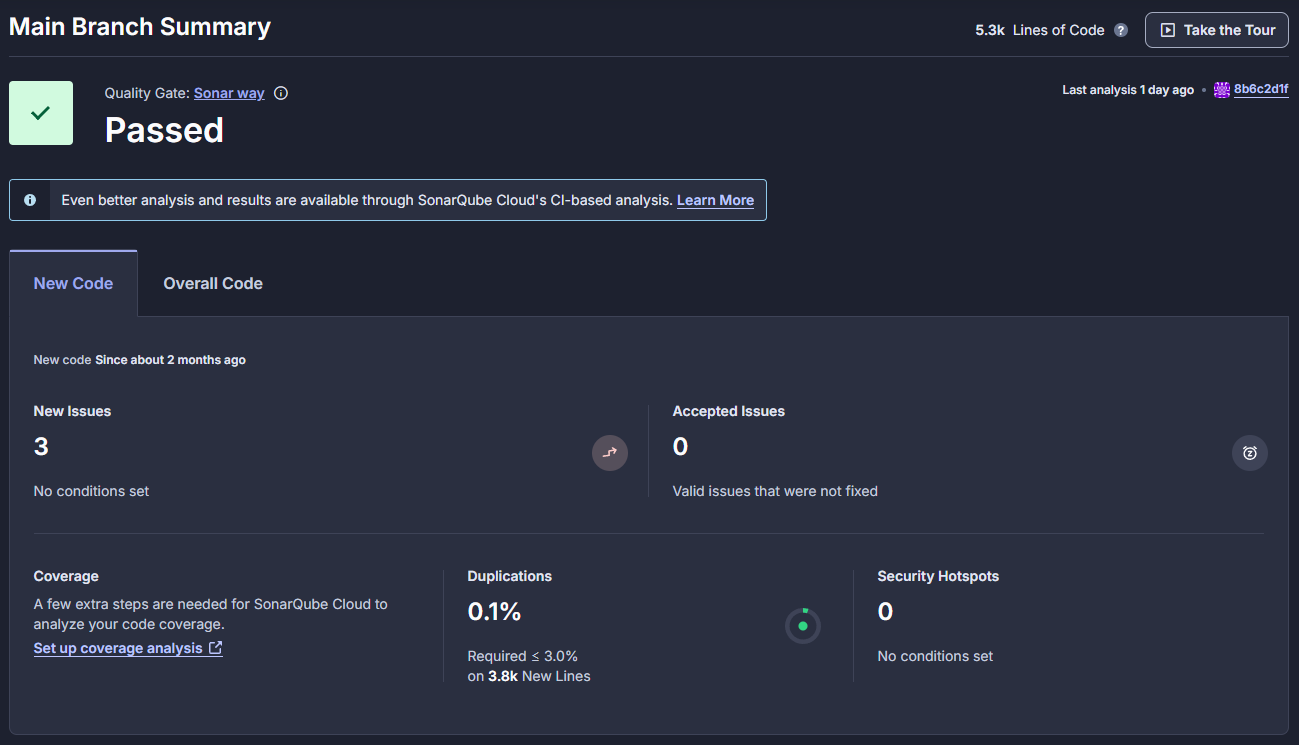
\includegraphics[width=\textwidth]{assets/code/sonarqube.png}
    }
    \caption{Schermata di Sonarqube Cloud}
    \label{fig:Sonarqube Cloud}
\end{figure}

\section{Testing dell'interfaccia utente}
Durante tutto lo sviluppo del frontend, sono state applicate le dieci regole
euristiche per l'usabilitá di Nielsen e Molich ed una checklist per l'usabilitá.

\subsection{Le dieci regole euristiche di Nielsen e Molich}

\subsubsection{Simple and Natural Dialogue}
Un esempio lampante di Simple and Natural Dialogue é la schermata di ricerca 
iniziale che nasconde funzionalità opzionali tramite l'utilizzo di menu dropdown,
risultando in un design semplice ed essenziale.

\begin{figure}[H]
  \adjustbox{width=1.4\textwidth,center}{
      \fbox{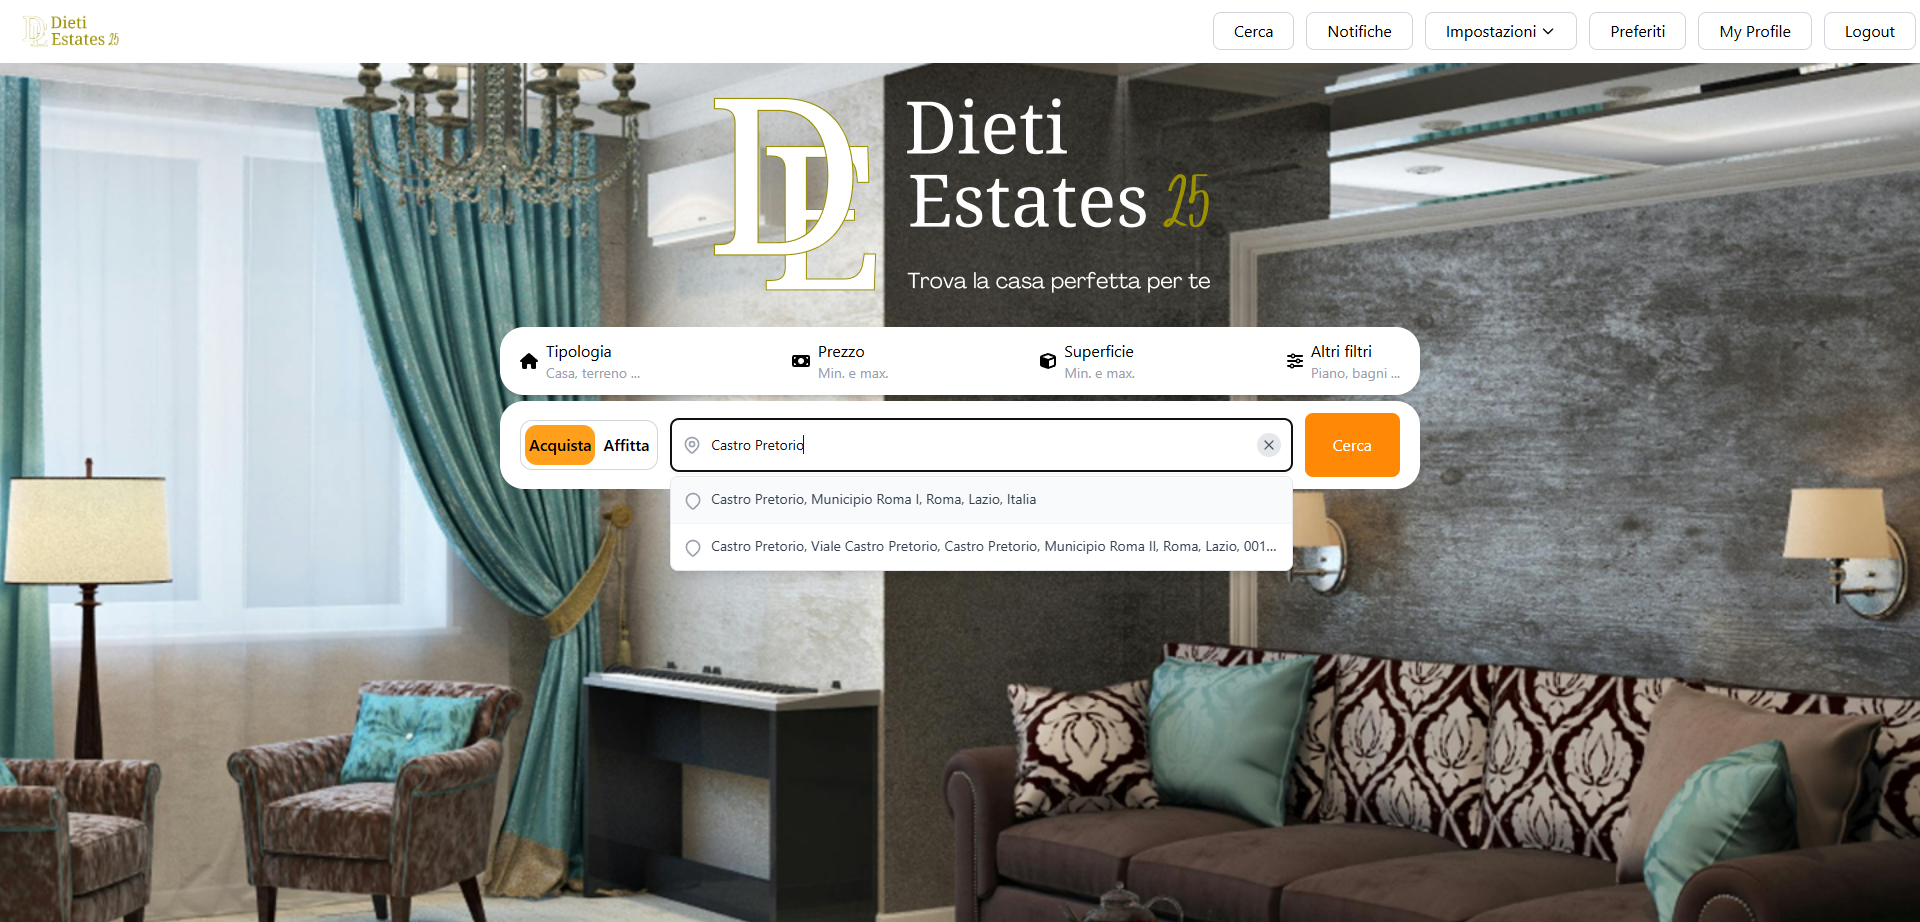
\includegraphics[width=\textwidth]{assets/frontend/home.png}}
  }
  \caption{Schermata home}
  \label{fig:schermata home}
\end{figure}

\subsubsection{Speak the User's Language}
L'interfaccia non fa mai uso di linguaggio tecnico informatico.

\begin{figure}[h]
  \adjustbox{width=1.4\textwidth,center}{
    \fbox{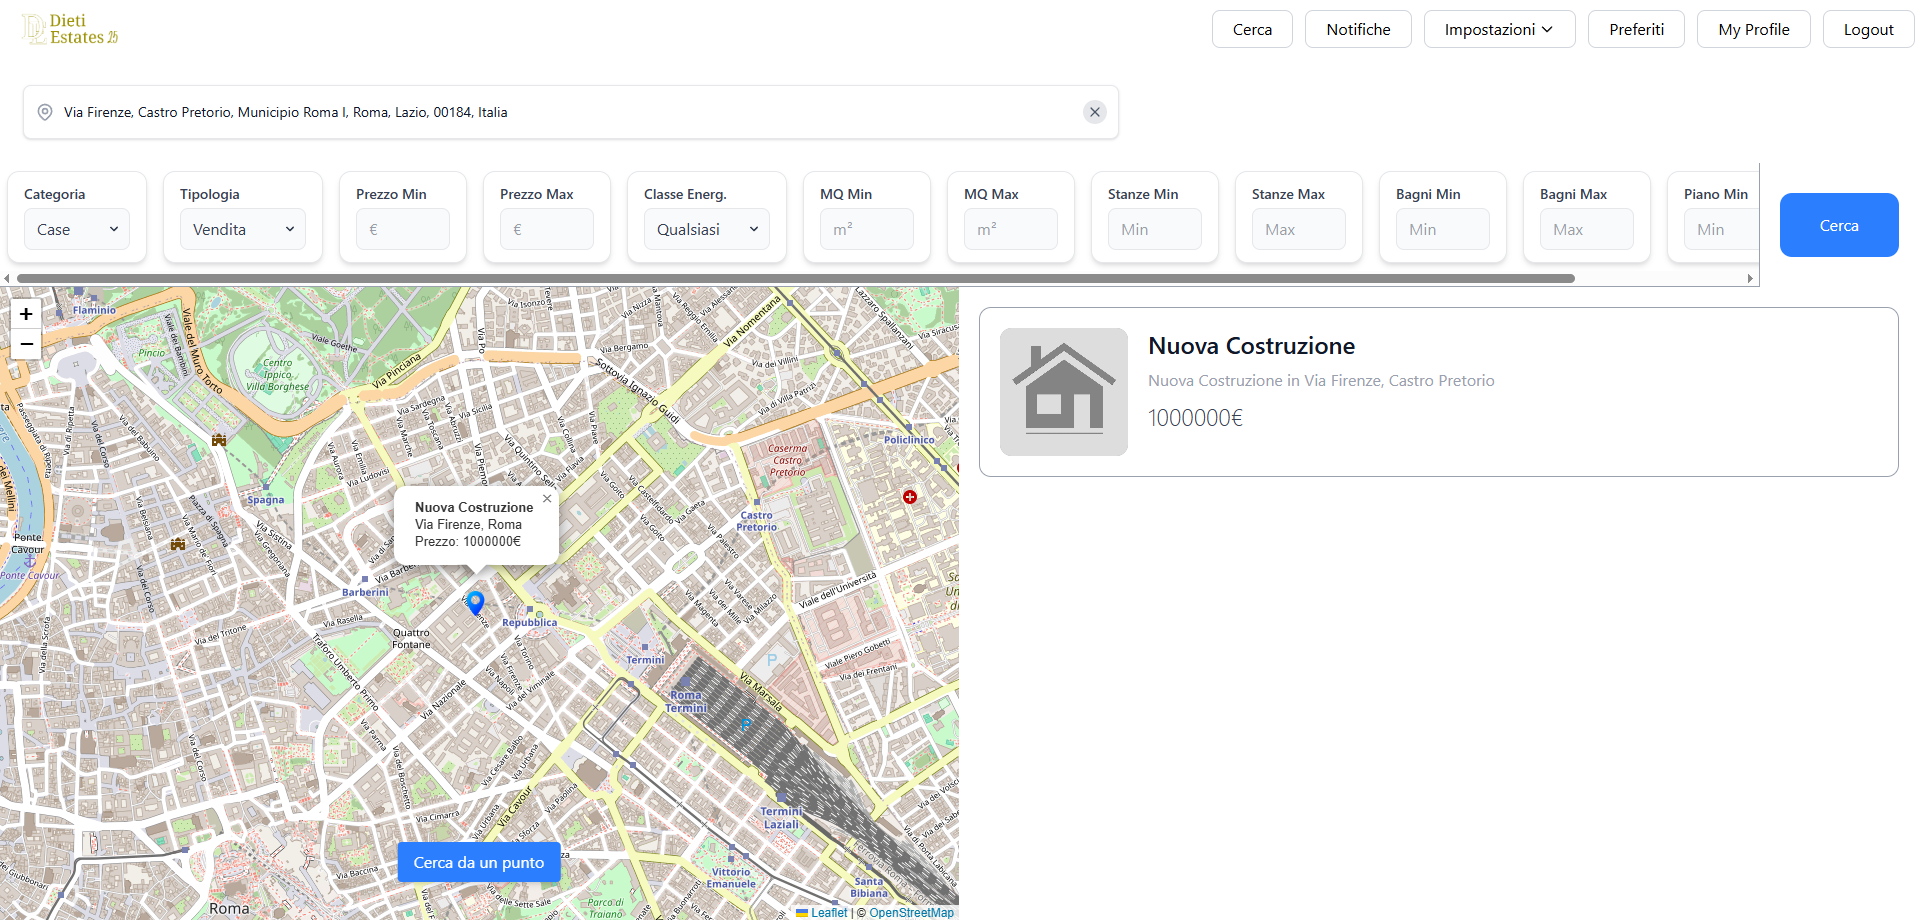
\includegraphics[width=\textwidth]{assets/frontend/cerca-annuncio.png}}
  }
  \caption{Schermata di ricerca}
  \label{fig:Schermata di ricerca}
\end{figure}

\begin{figure}[h]
  \adjustbox{width=1.4\textwidth,center}{
    \fbox{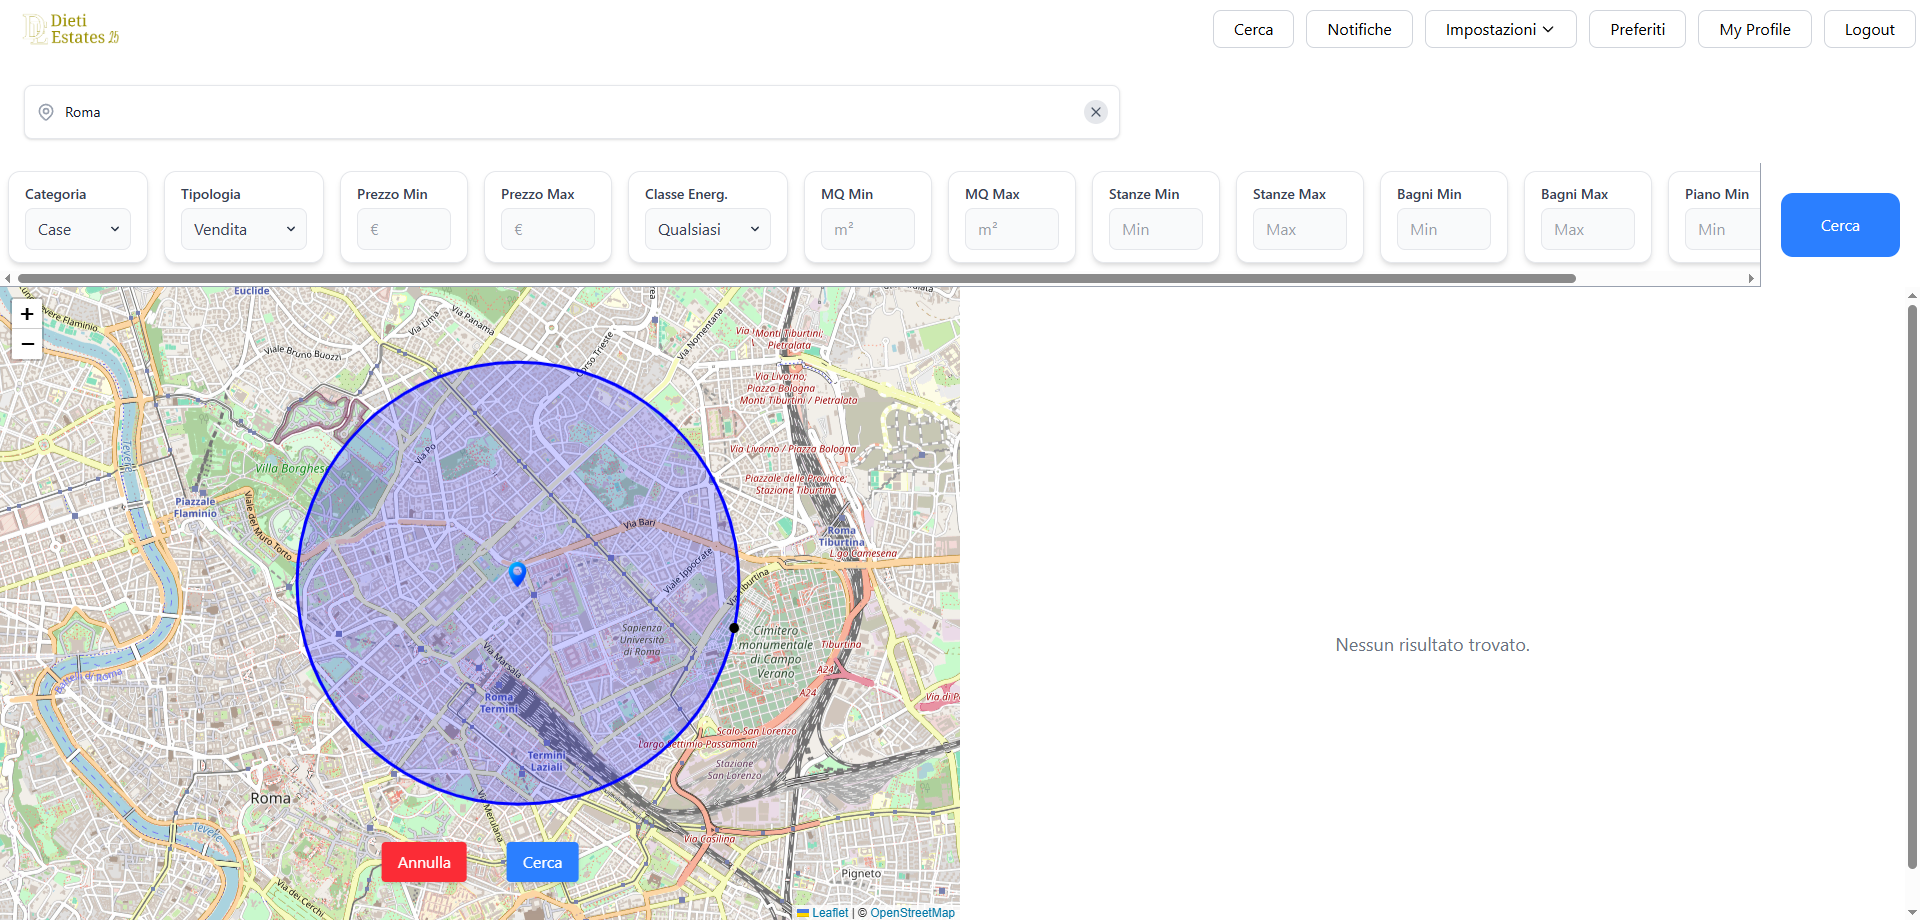
\includegraphics[width=\textwidth]{assets/frontend/cerca-annuncio-tramite-raggio.png}}
  }
  \caption{Schermata di ricerca con raggio}
  \label{fig:Schermata di ricerca con raggio}
\end{figure}

\subsubsection{Consistency}
Parlando di consistenza interna - la consistenza tra i vari componenti dell'interfaccia -, 
le schermate sono state fattorizzate il piú possibile, in modo tale da
rendere le operazioni prevedibili dal punto di vista dell'utente.

Per quanto riguarda la consistenza esterna - la consistenza dell'interfaccia con
le convenzioni che vigono nel mondo -, ci siamo adattati quanto possibile a piattaforme
note del settore come Immobiliare.it.

\begin{figure}[h]
  \adjustbox{width=1.4\textwidth,center}{
    \fbox{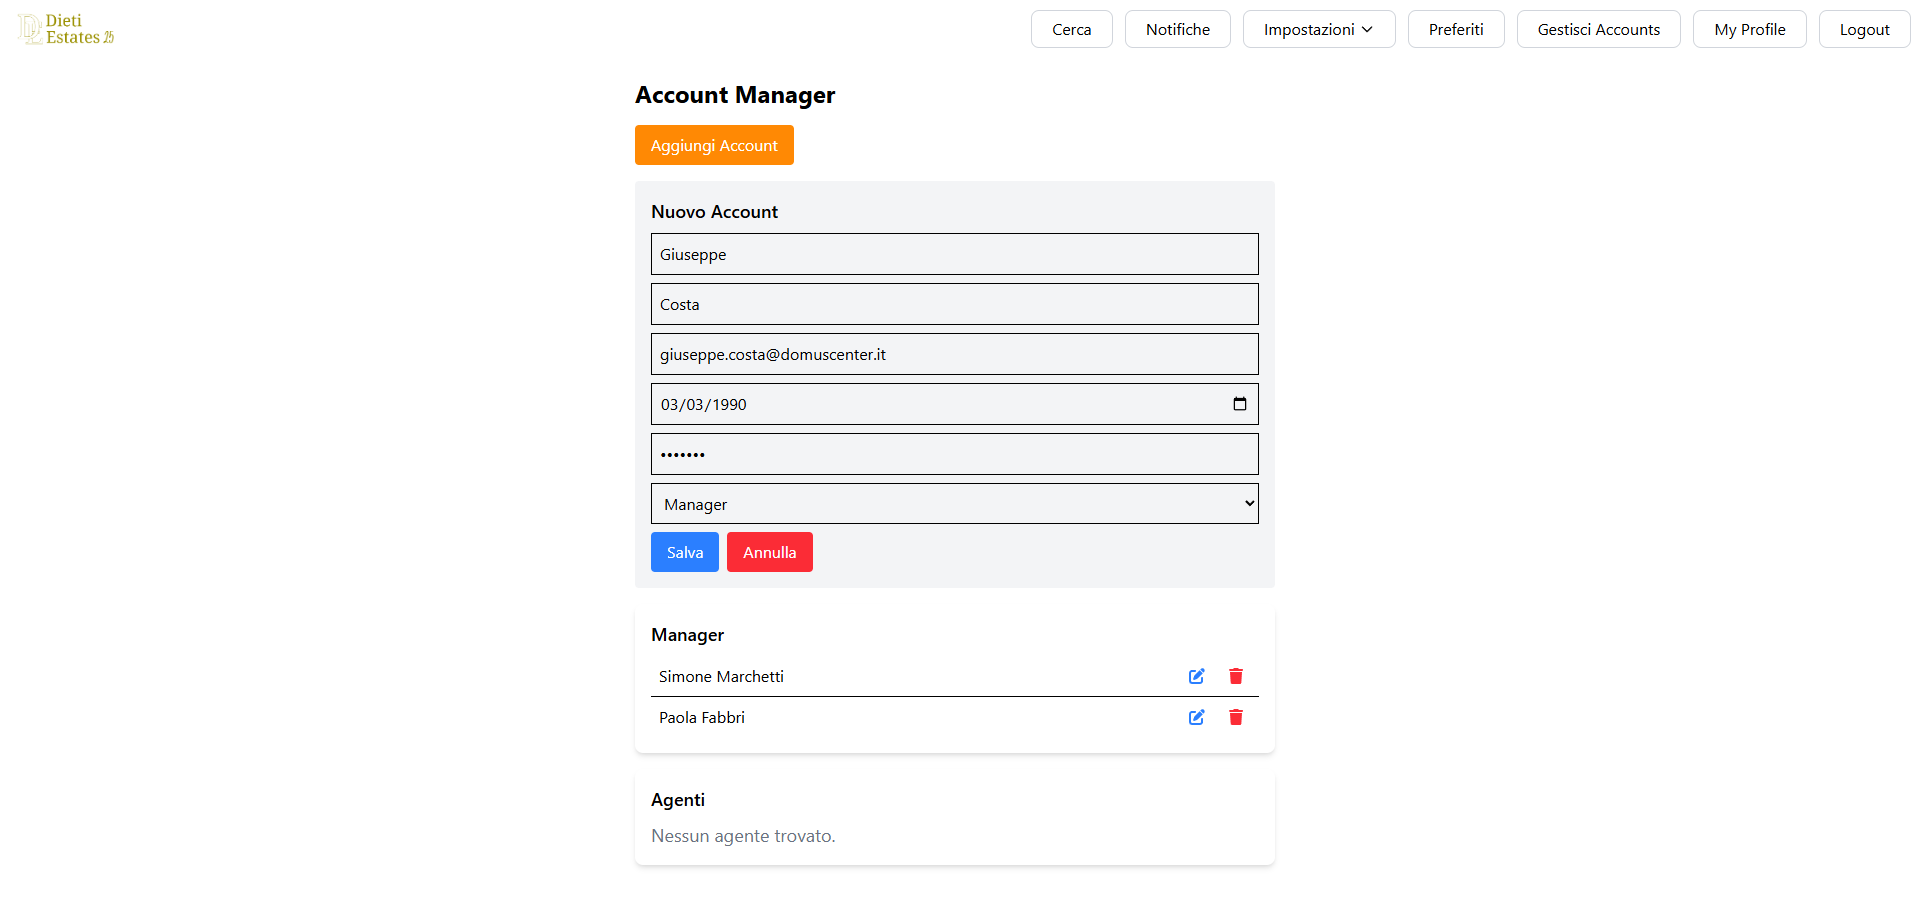
\includegraphics[width=\textwidth]{assets/frontend/create-manager.png}}
  }
  \caption{Schermata di crezione di un account manager}
  \label{fig:Schermata di crezione di un account manager}
\end{figure}

\subsubsection{Feedback}
Il sistema informa continuamente gli utenti sui risultati delle loro azioni sia con 
esito positivo che negativo.

\begin{figure}[h]
  \adjustbox{width=1.4\textwidth,center}{
    \fbox{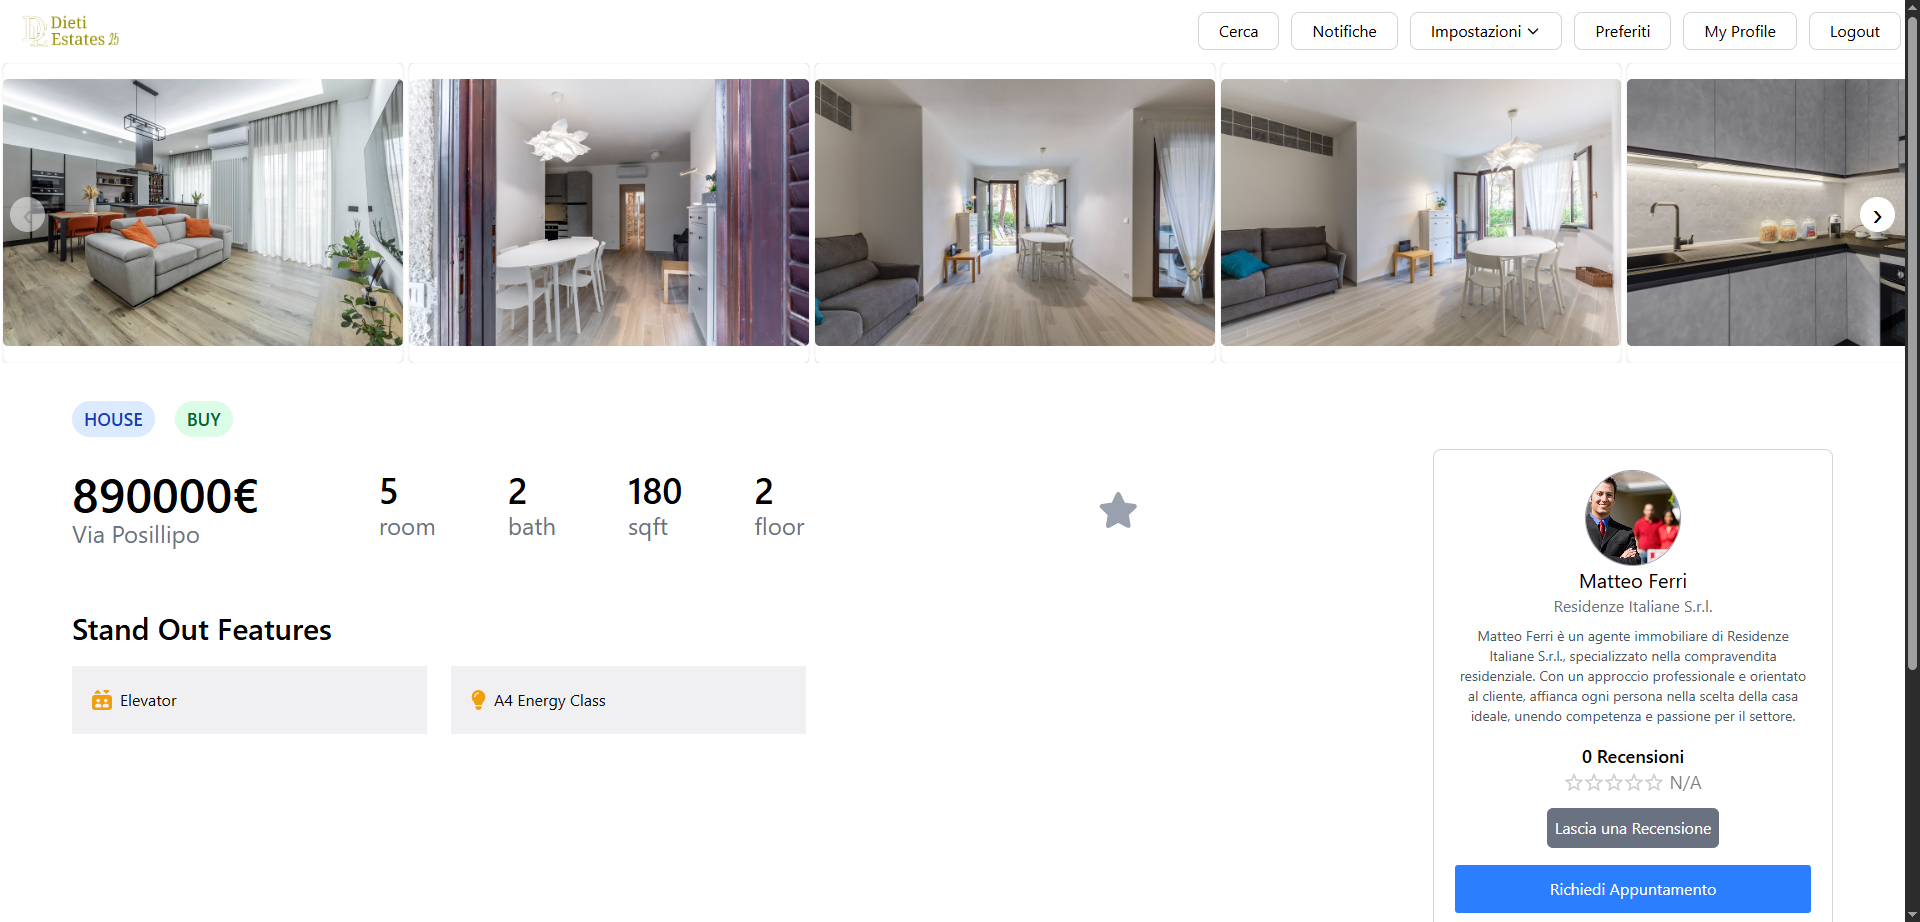
\includegraphics[width=\textwidth]{assets/frontend/annuncio-specifico.png}}
  }
  \caption{Schermata di un annuncio specifico}
  \label{fig:Schermata di un annuncio specifico}
\end{figure}

\begin{figure}[h]
  \adjustbox{width=1.4\textwidth,center}{
    \fbox{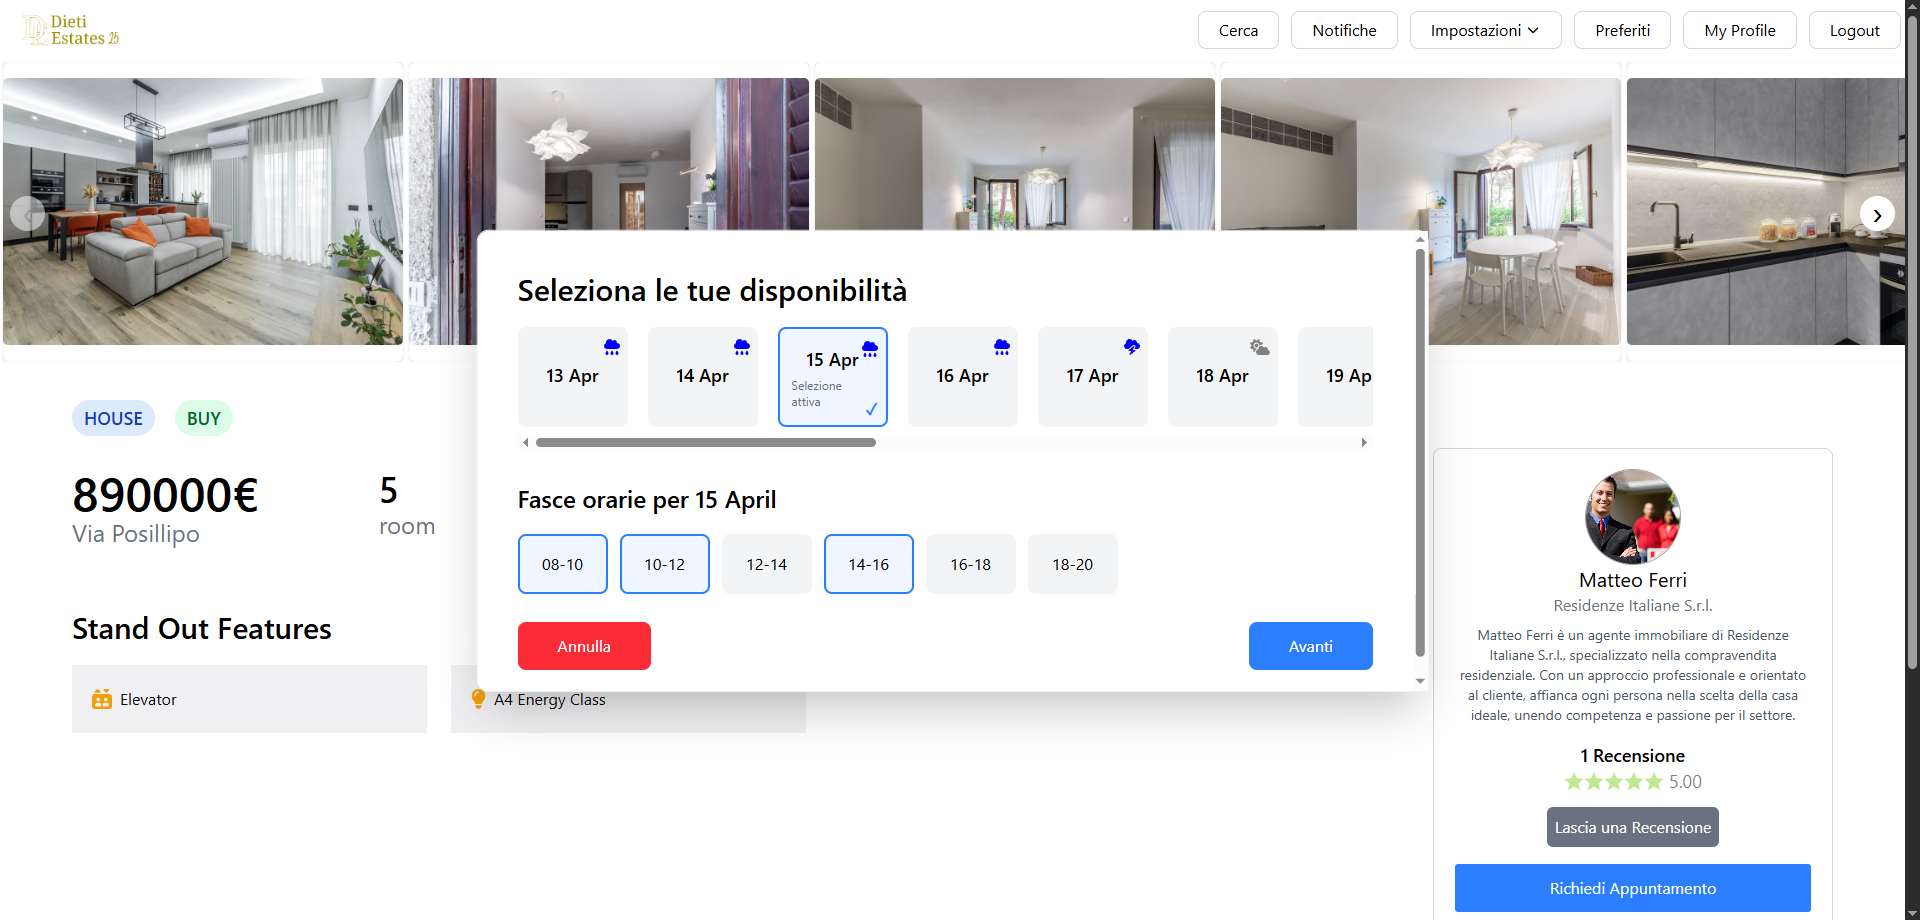
\includegraphics[width=\textwidth]{assets/frontend/richiedi-visita.png}}
  }
  \caption{Schermata di richiesta di visita}
  \label{fig:Schermata di richiesta di visita}
\end{figure}

\begin{figure}[h]
  \adjustbox{width=1.4\textwidth,center}{
    \fbox{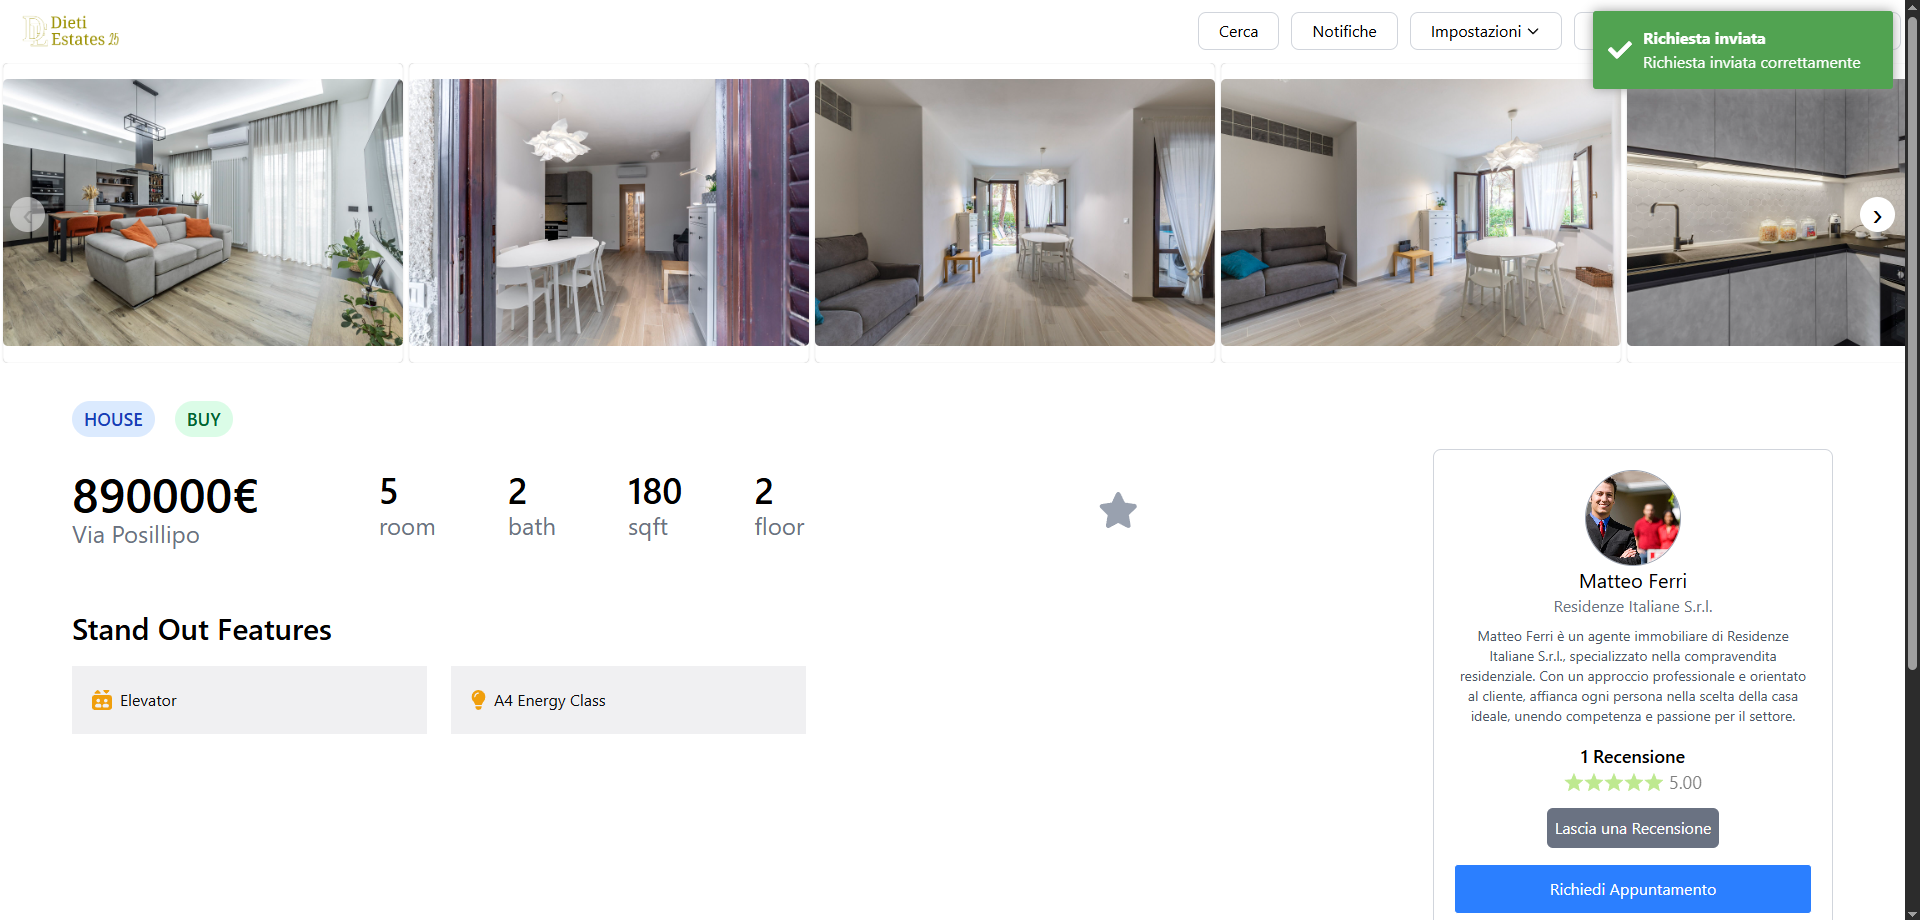
\includegraphics[width=\textwidth]{assets/frontend/feedback.png}}
  }
  \caption{feedback}
  \label{fig:feedback}
\end{figure}

\begin{figure}[h]
  \adjustbox{width=1.4\textwidth,center}{
    \fbox{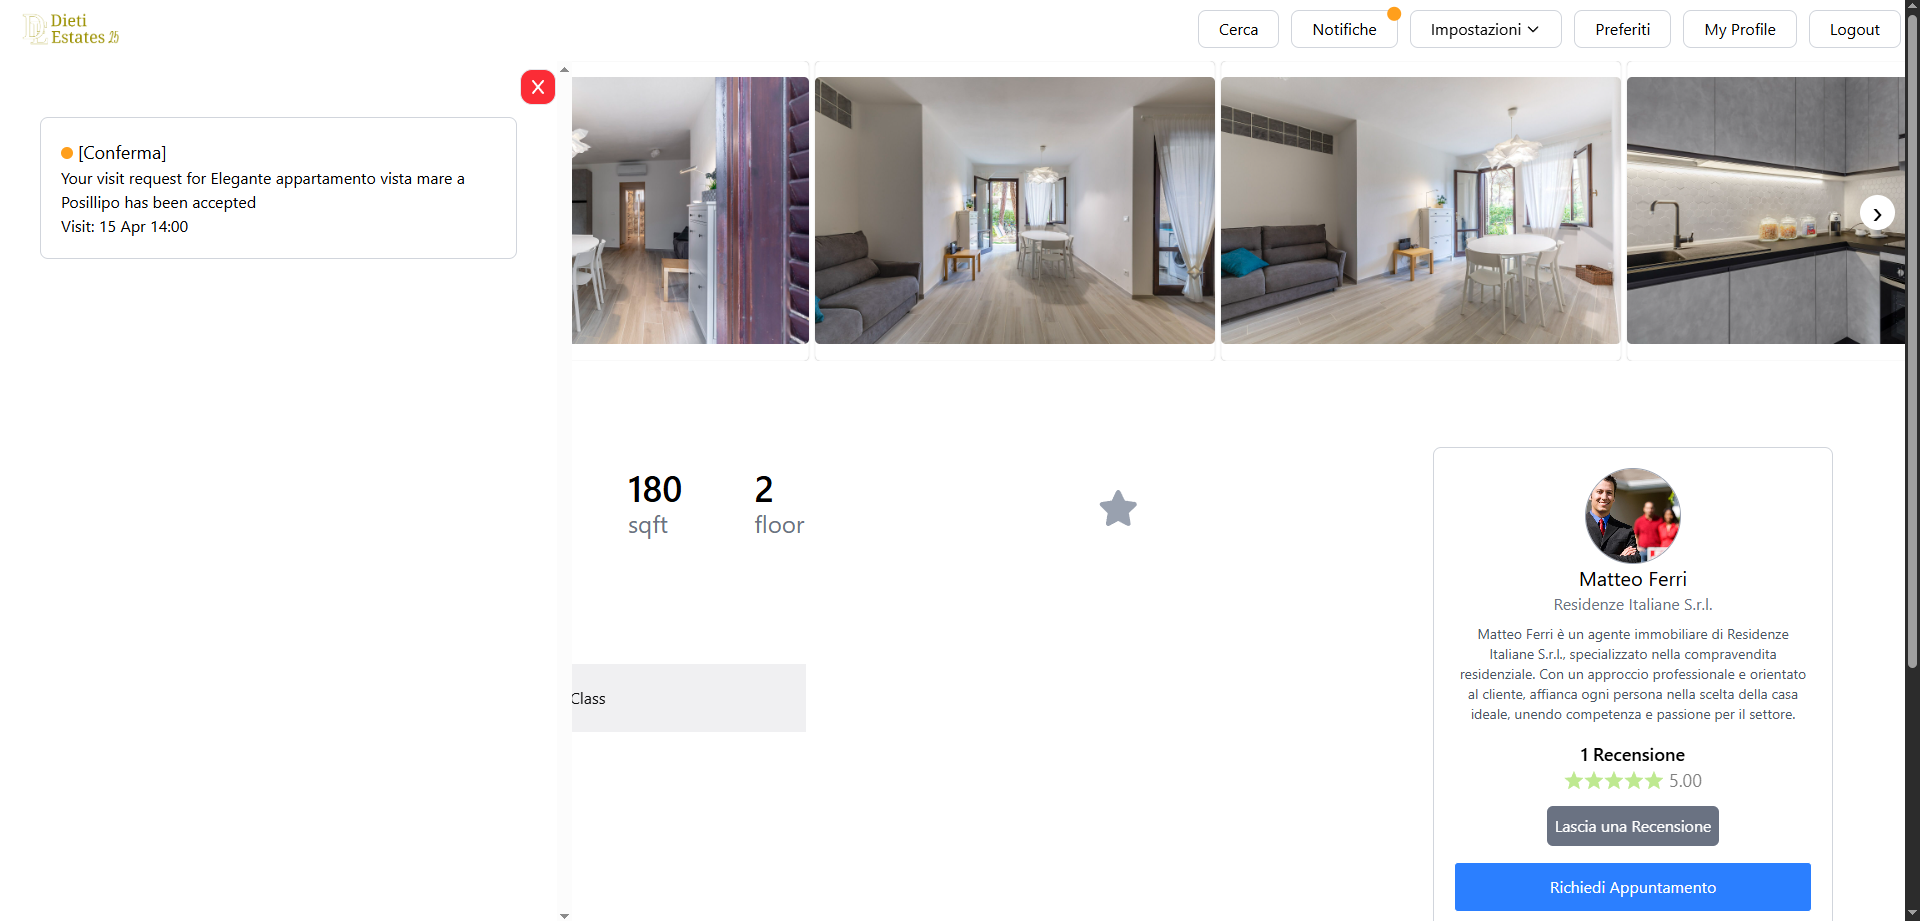
\includegraphics[width=\textwidth]{assets/frontend/notifiche.png}}
  }
  \caption{Sidebar delle notifiche}
  \label{fig:Sidebar delle notifiche}
\end{figure}

\begin{figure}[h]
  \adjustbox{width=1.4\textwidth,center}{
    \fbox{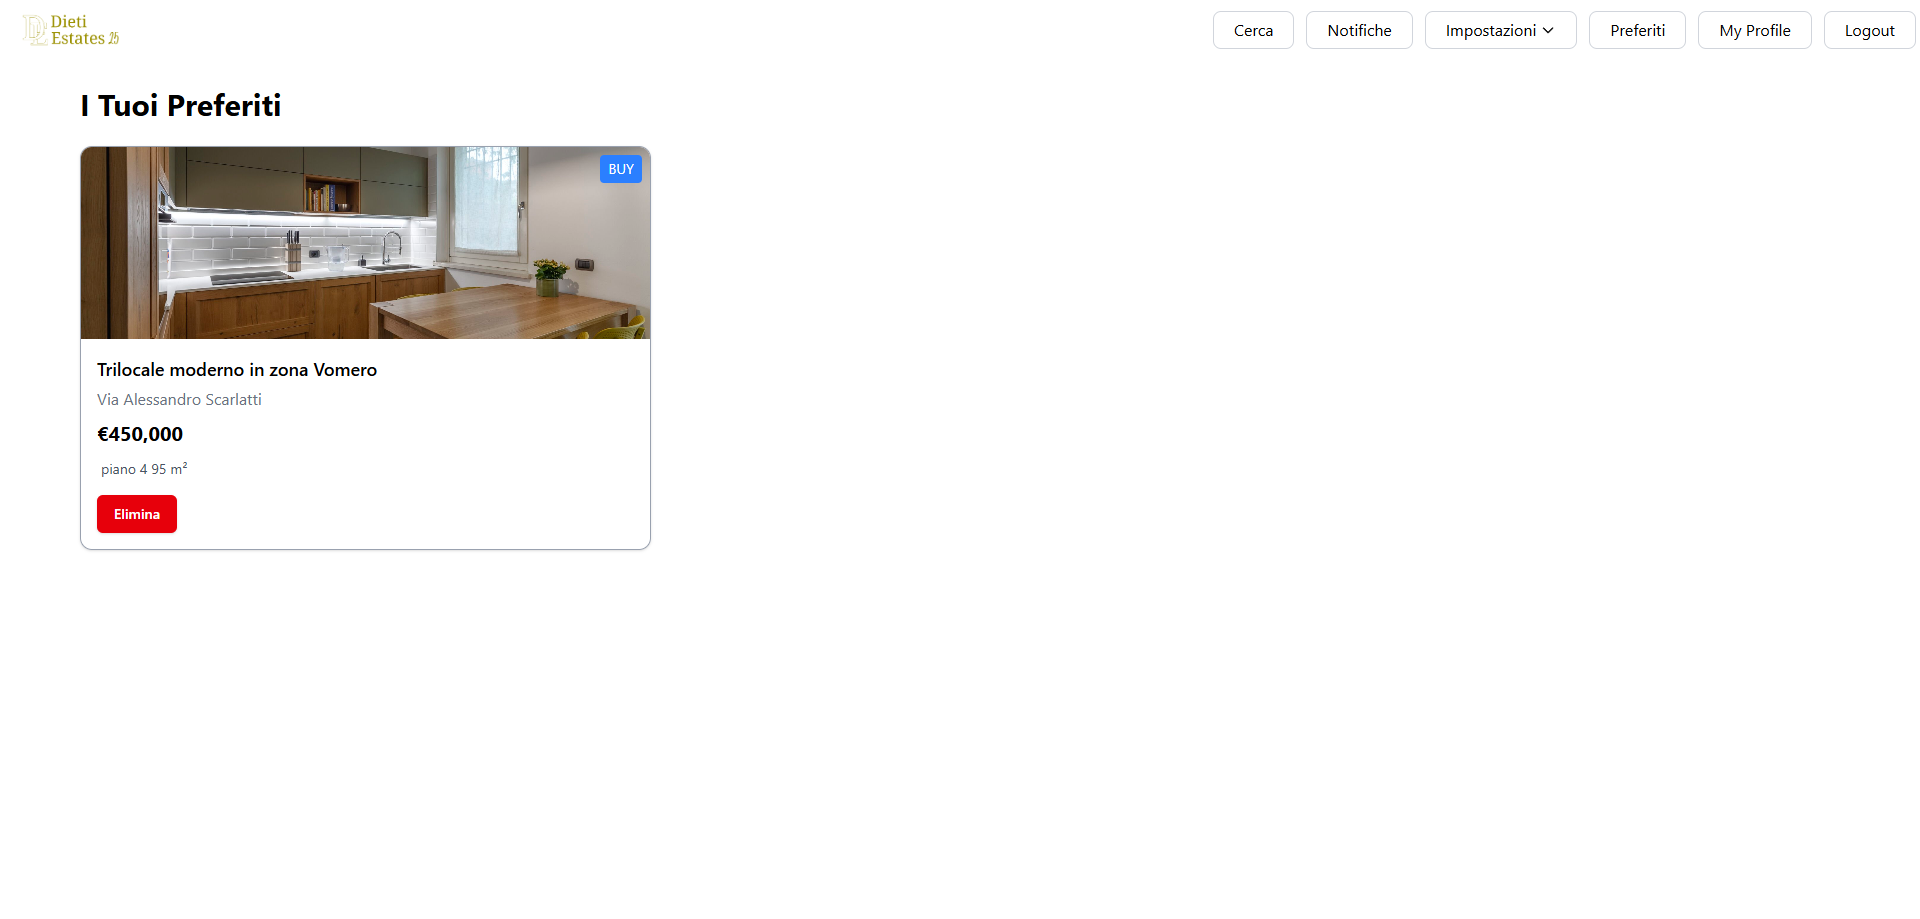
\includegraphics[width=\textwidth]{assets/frontend/preferiti.png}}
  }
  \caption{Schermata degli annunci preferiti}
  \label{fig:Schermata degli annunci preferiti}
\end{figure}

\begin{figure}[h]
  \adjustbox{width=1.4\textwidth,center}{
    \fbox{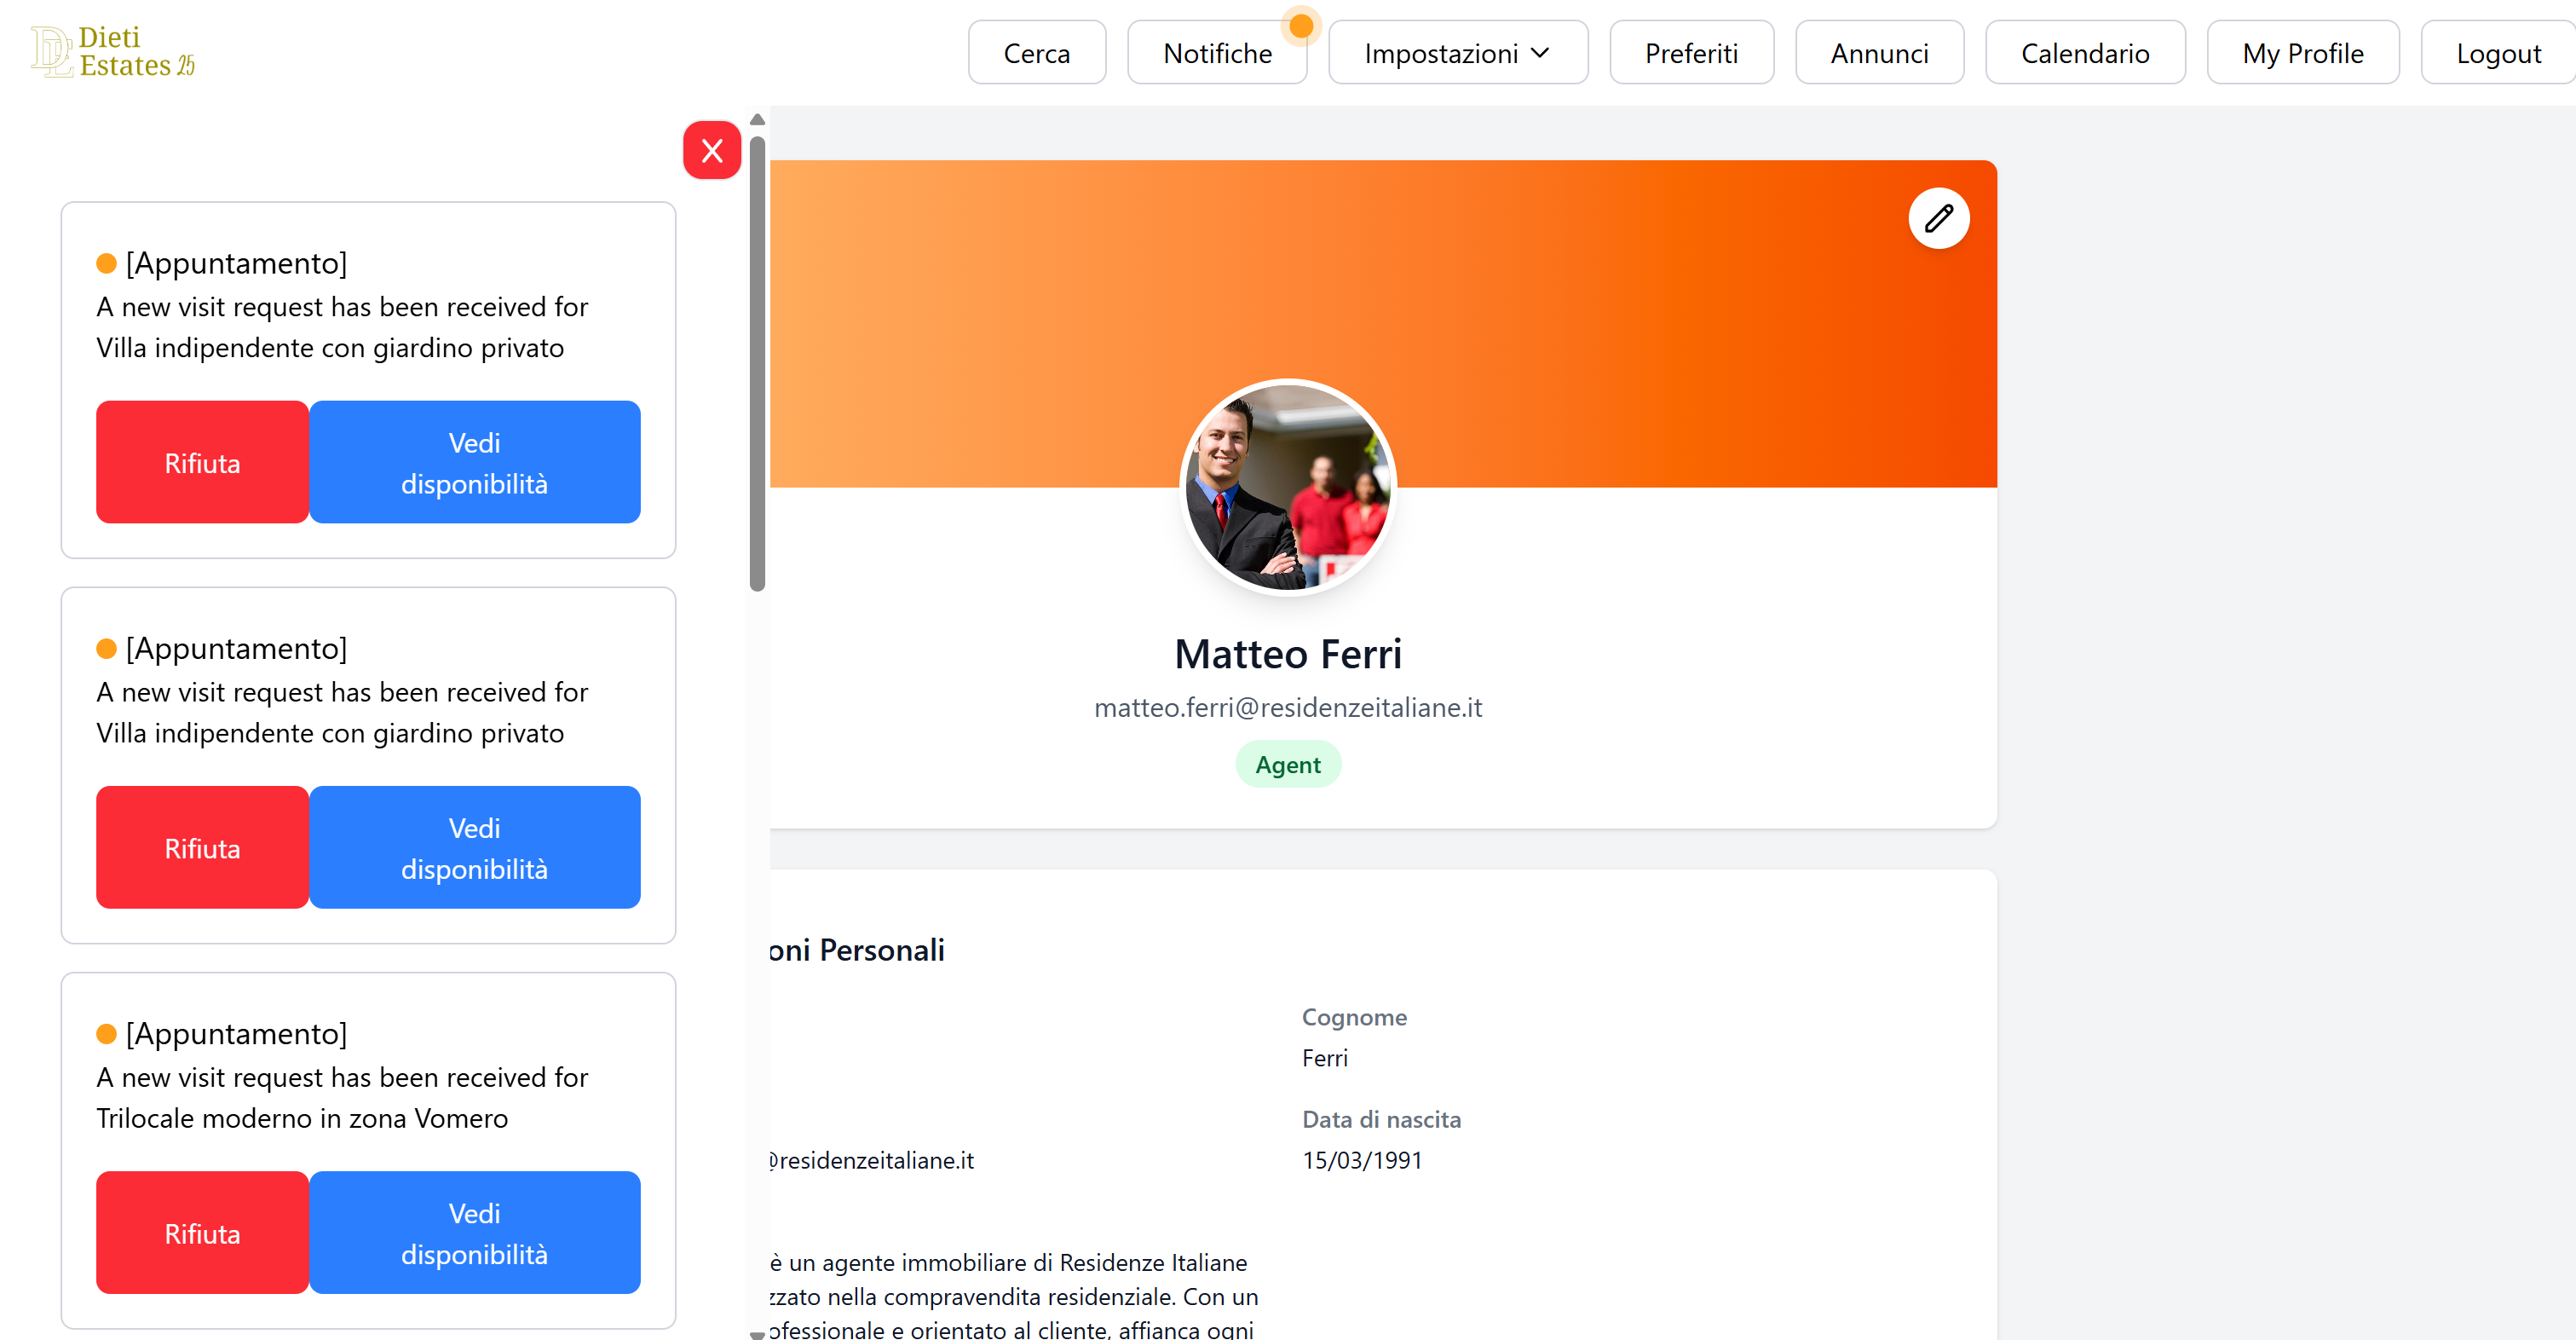
\includegraphics[width=\textwidth]{assets/frontend/notifiche-agente.png}}
  }
  \caption{Sidebar delle notifiche dell'agente}
  \label{fig:Sidebar delle notifiche dell'agente}
\end{figure}

\begin{figure}[h]
  \adjustbox{width=1.4\textwidth,center}{
    \fbox{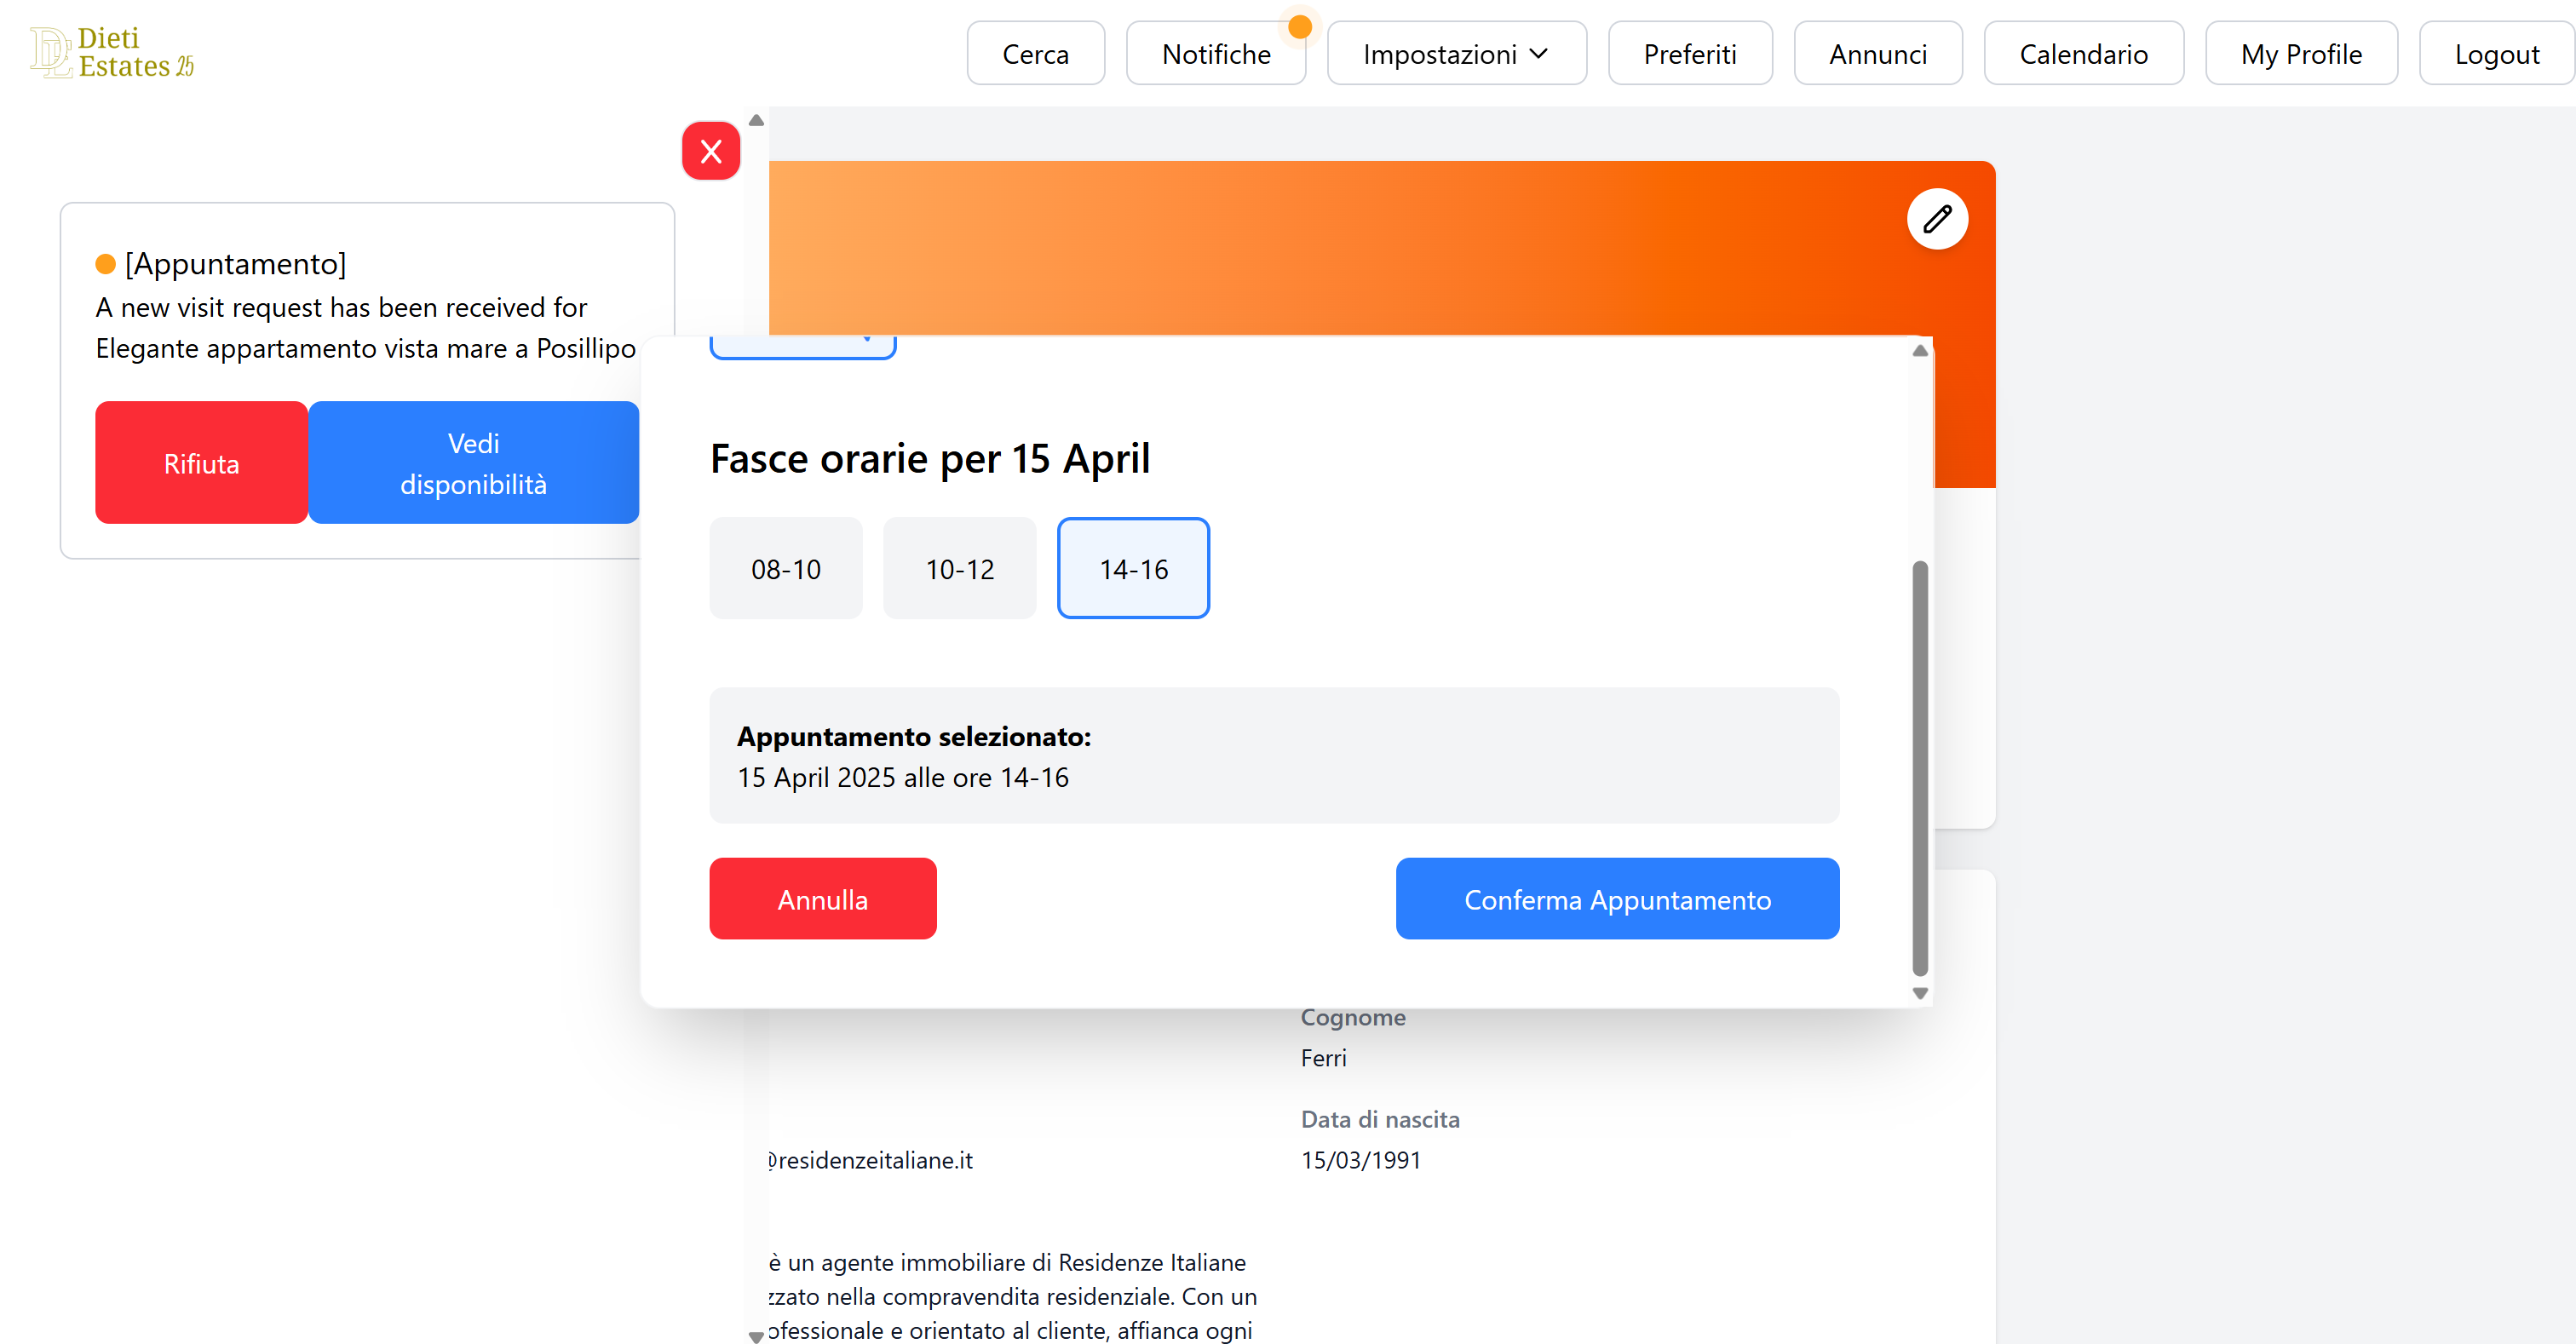
\includegraphics[width=\textwidth]{assets/frontend/conferma-appuntamento.png}}
  }
  \caption{Schermata di conferma appuntamento}
  \label{fig:Schermata di conferma appuntamento}
\end{figure}

\begin{figure}[h]
  \adjustbox{width=1.4\textwidth,center}{
    \fbox{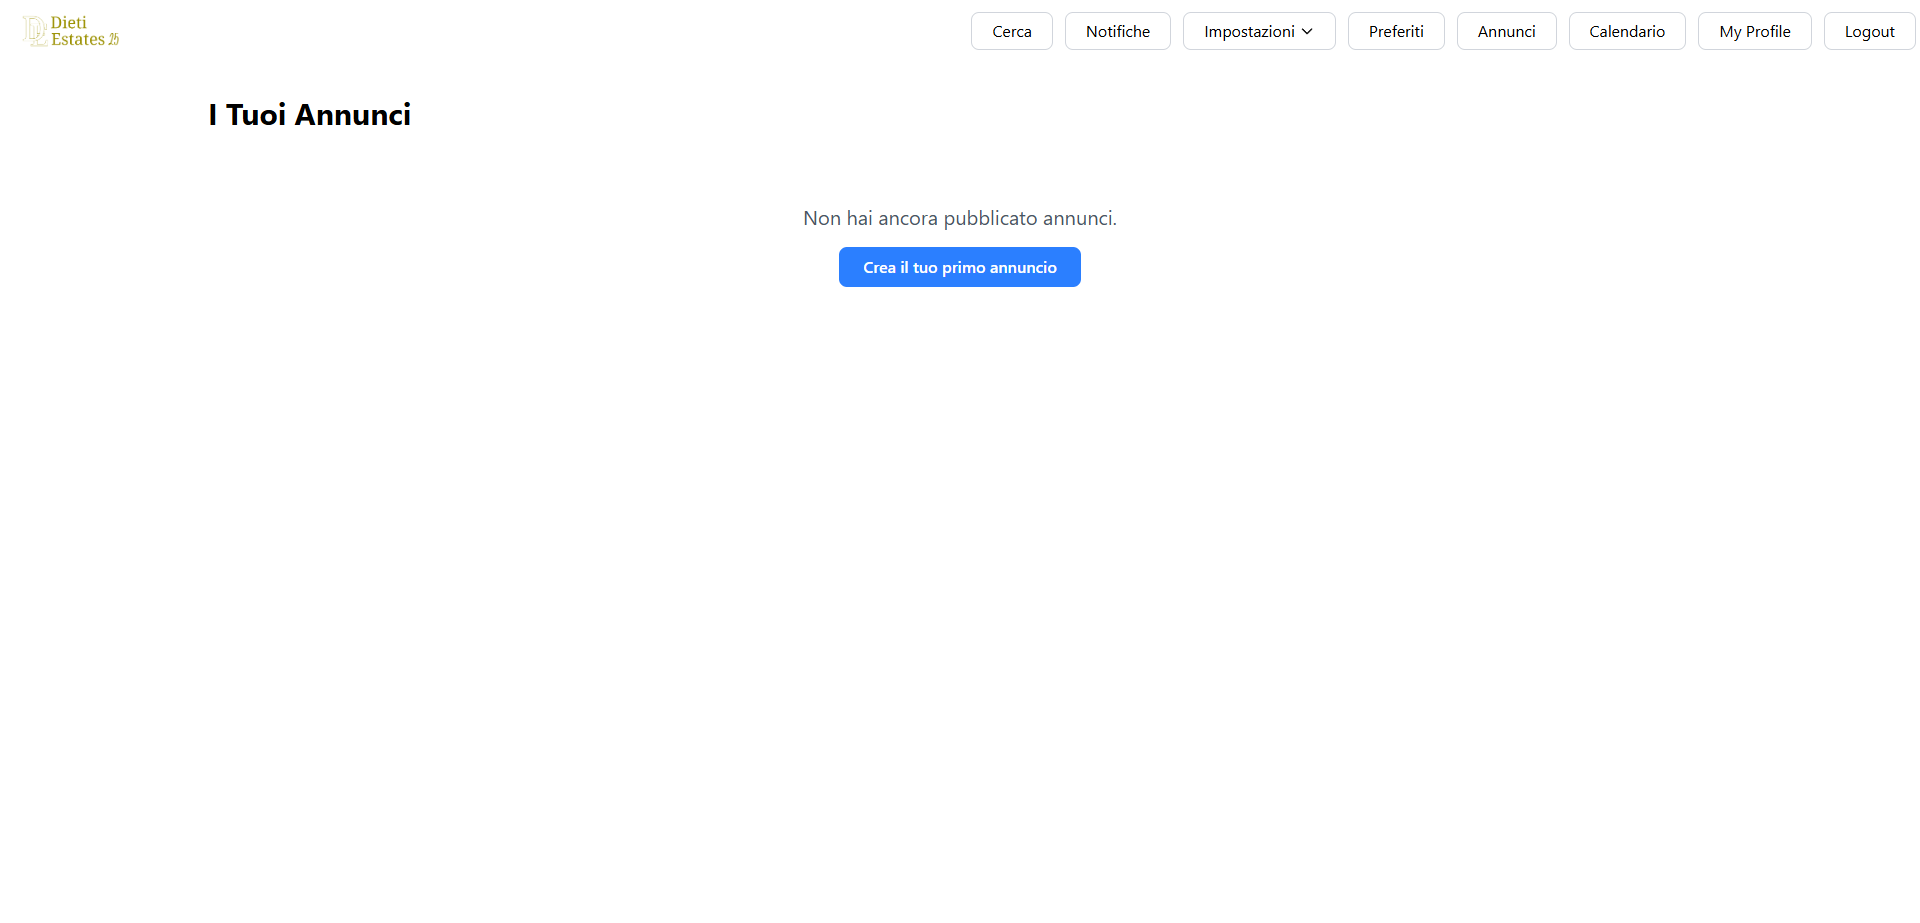
\includegraphics[width=\textwidth]{assets/frontend/i-tuoi-annunci-blank.png}}
  }
  \caption{Schermata vuota "i tuoi annunci"}
  \label{fig:Schermata vuota "i tuoi annunci"}
\end{figure}

\begin{figure}[h]
  \adjustbox{width=1.4\textwidth,center}{
    \fbox{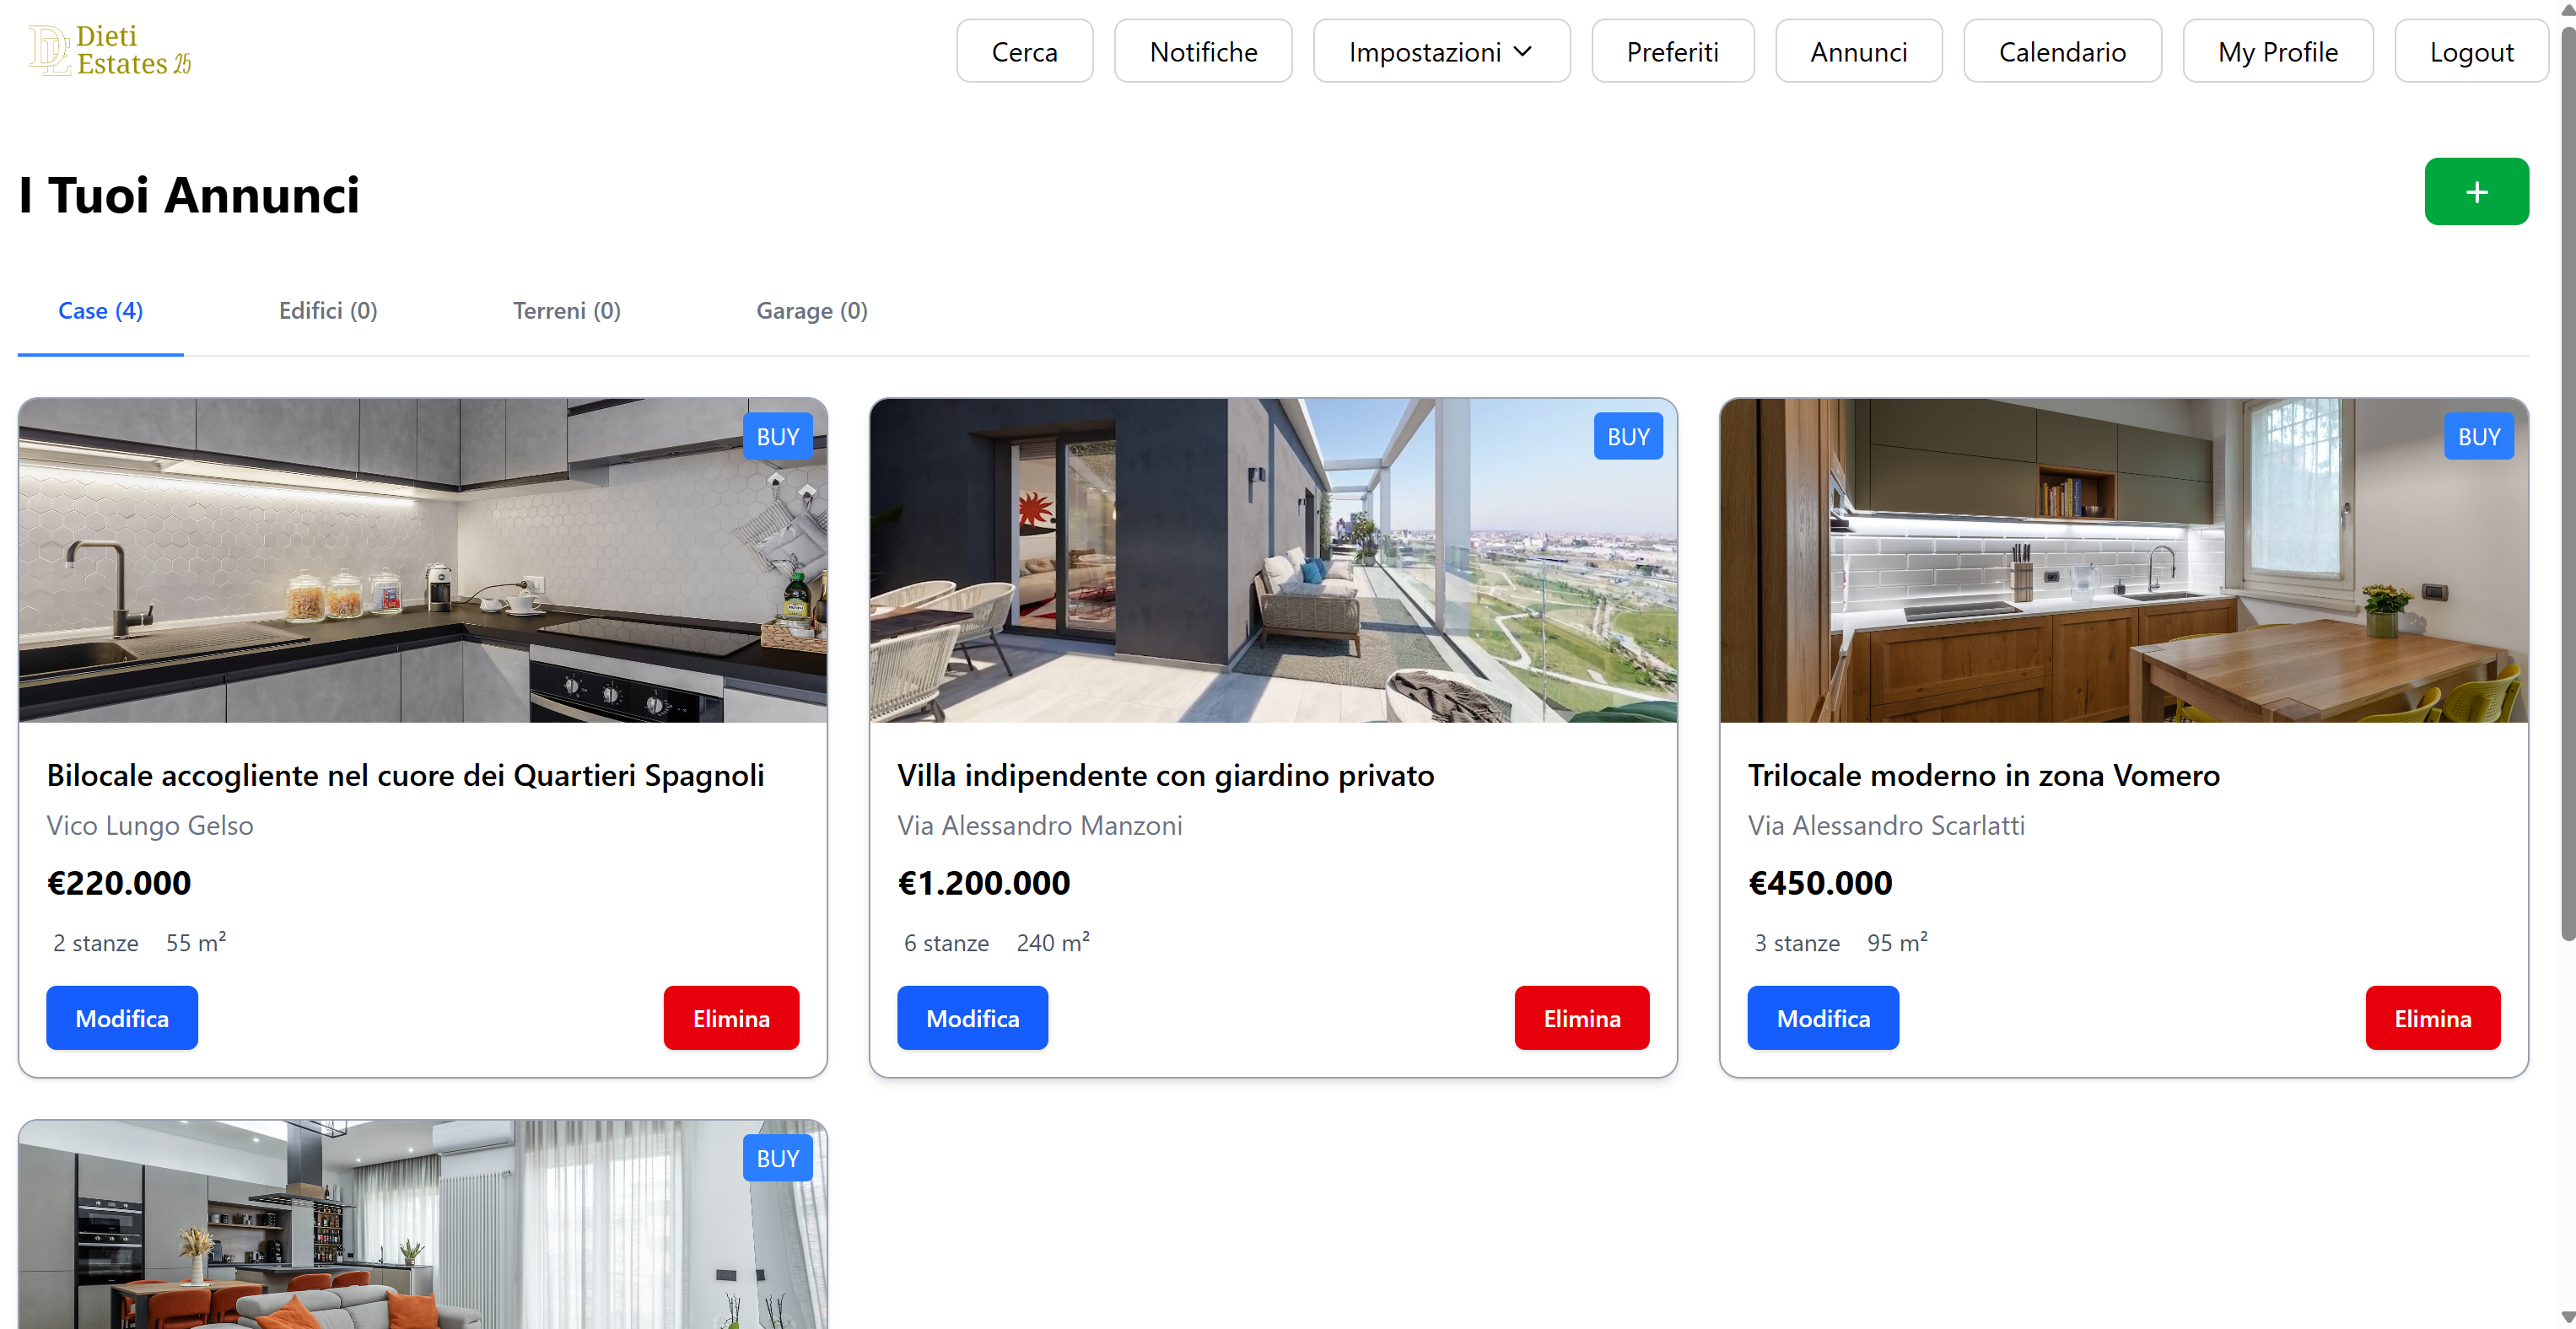
\includegraphics[width=\textwidth]{assets/frontend/i-tuoi-annunci.png}}
  }
  \caption{Schermata "i tuoi annunci"}
  \label{fig:Schermata tuoi annunci}
\end{figure}

\begin{figure}[h]
  \adjustbox{width=1.4\textwidth,center}{
    \fbox{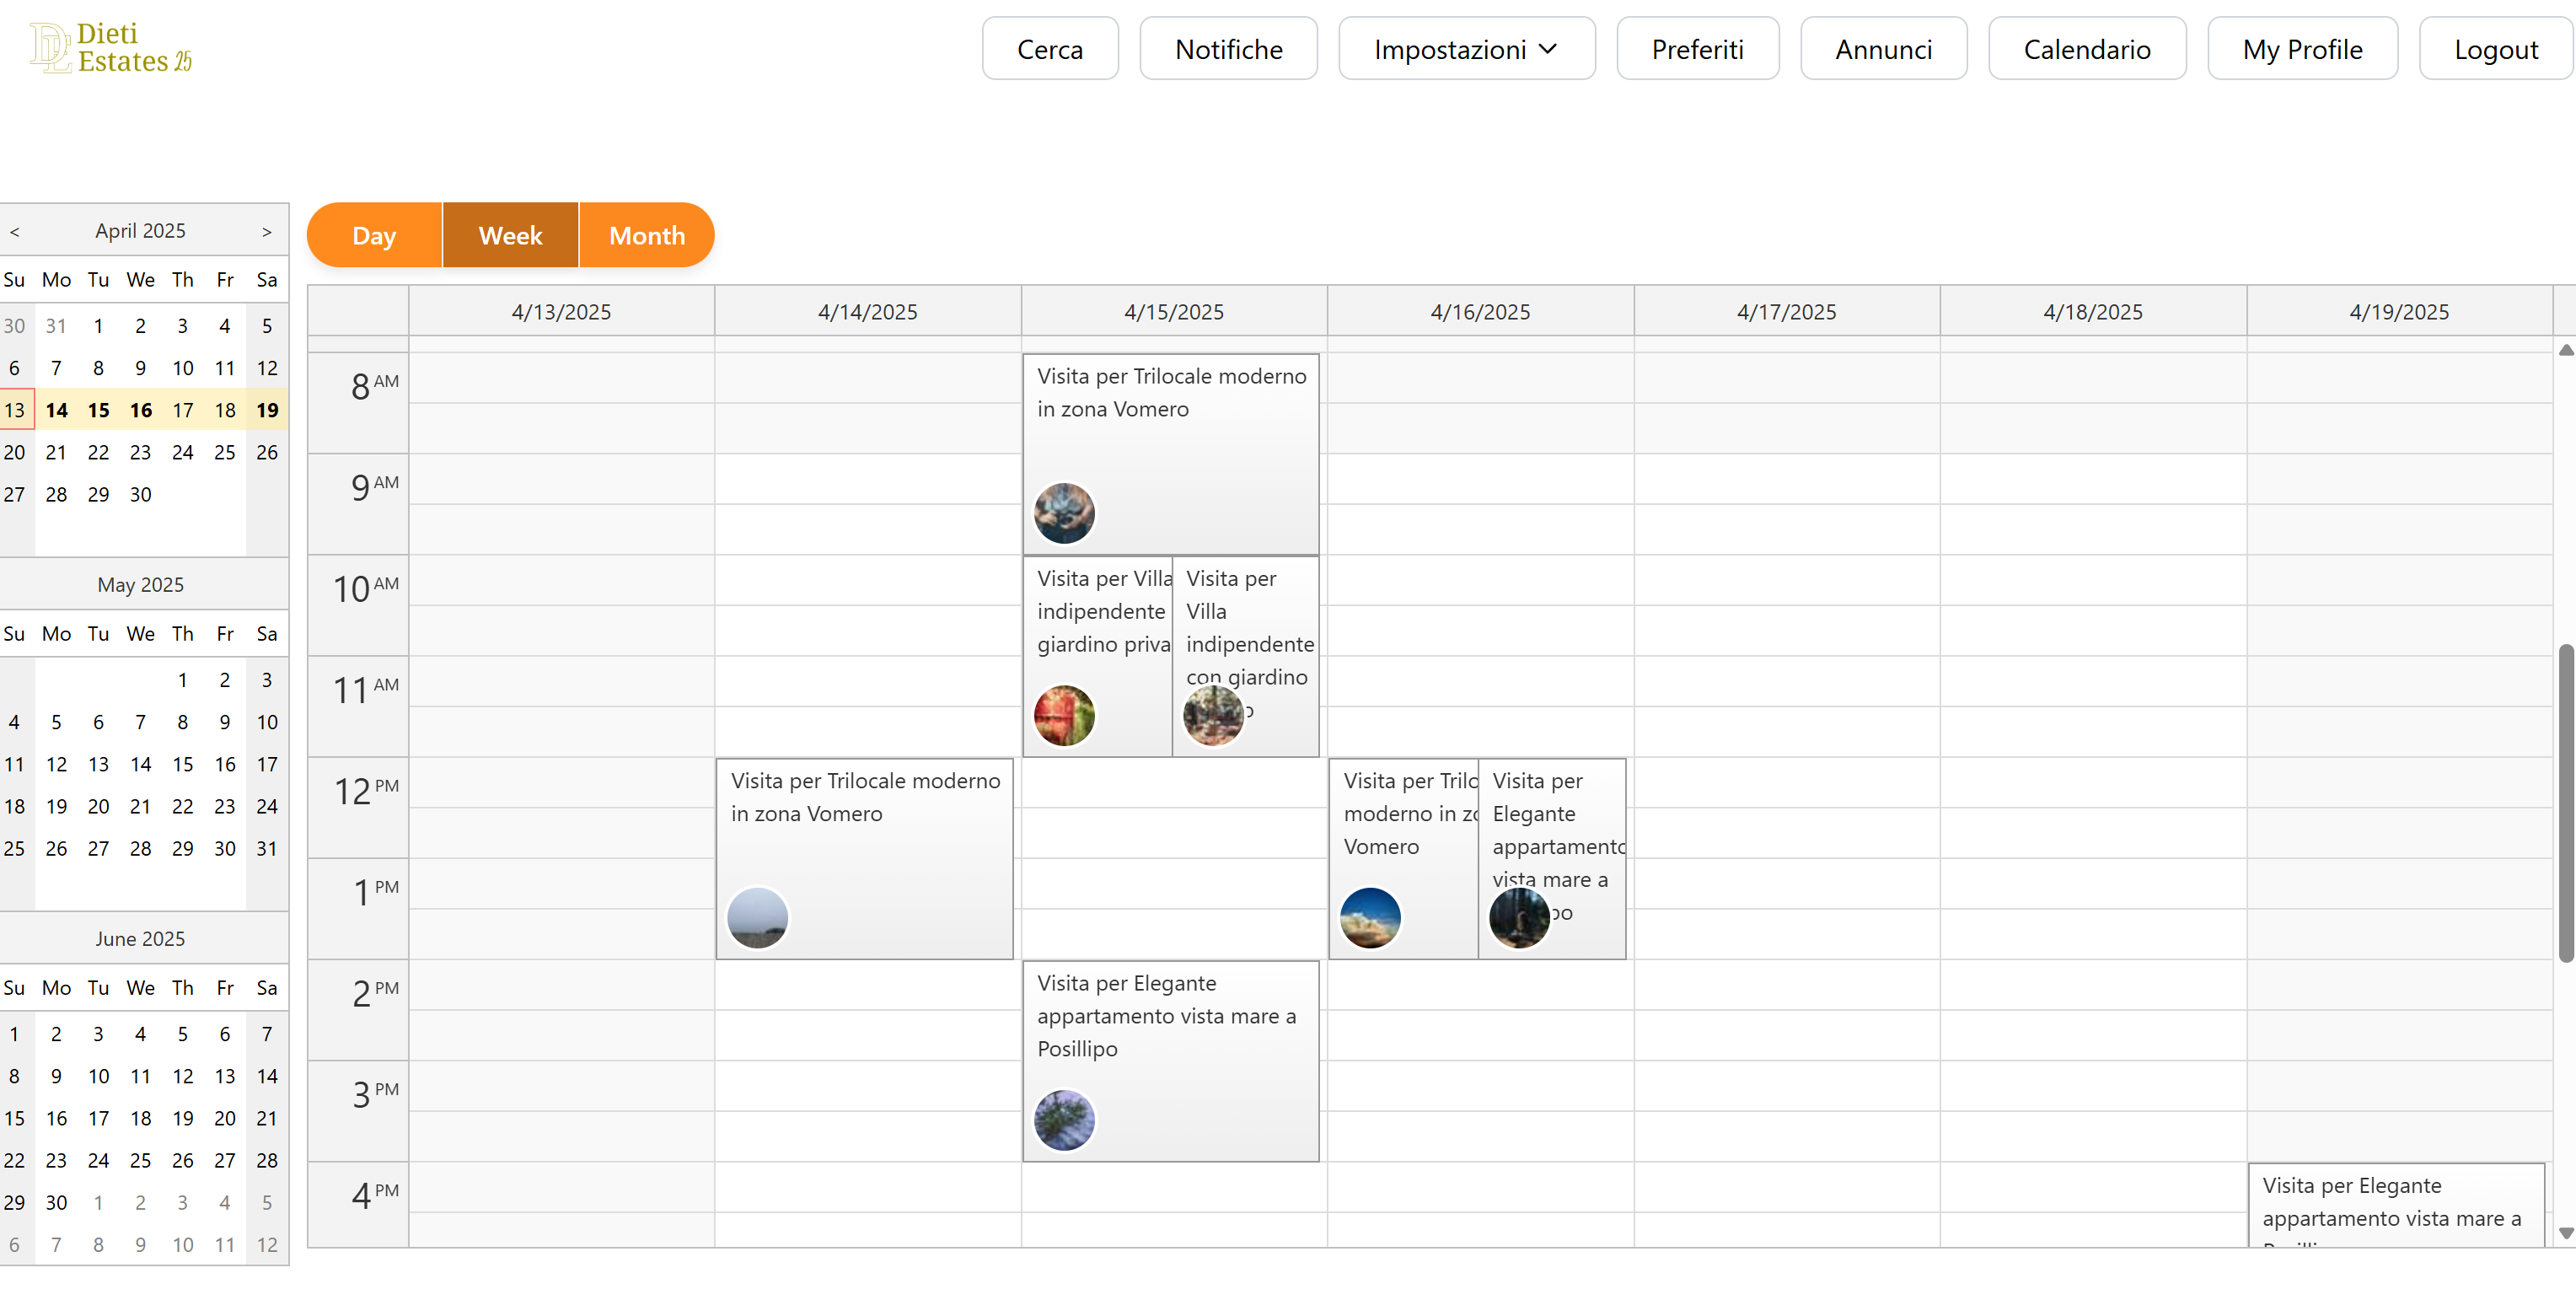
\includegraphics[width=\textwidth]{assets/frontend/calendario-agente.png}}
  }
  \caption{Il calendario dell'agente}
  \label{fig:Il calendario dell'agente}
\end{figure}

\begin{figure}[h]
  \adjustbox{width=1.4\textwidth,center}{
      \fbox{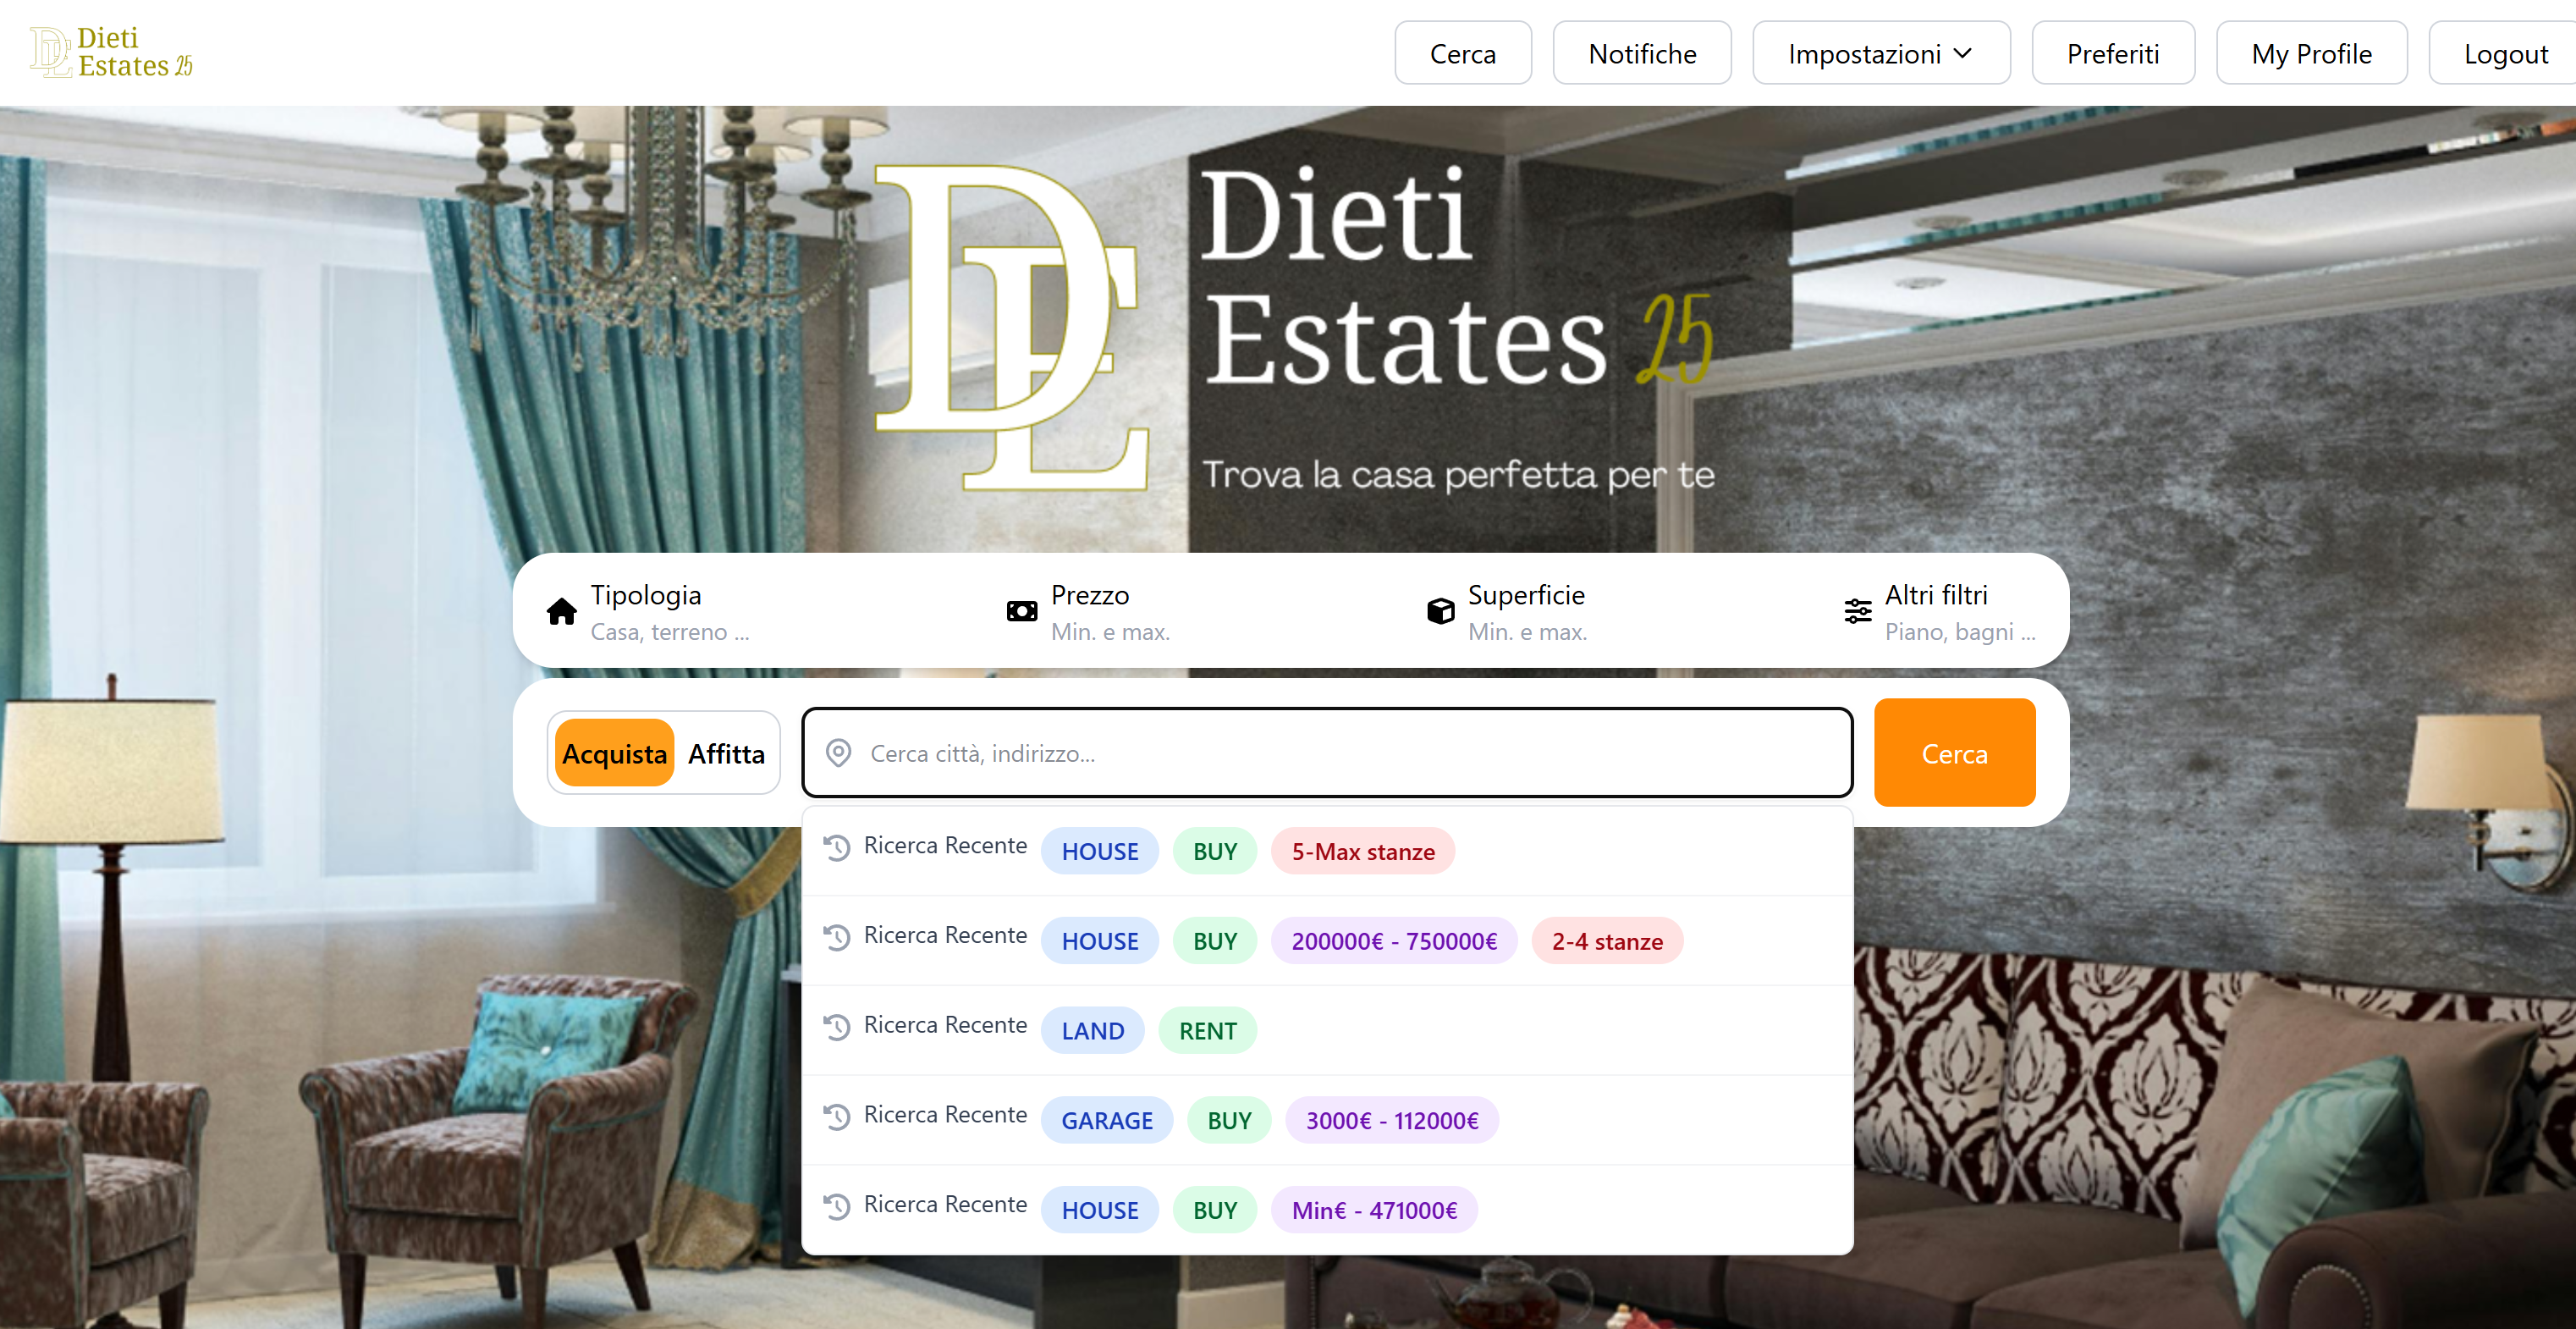
\includegraphics[width=\textwidth]{assets/frontend/ricerche-recenti.png}}
  }
  \caption{Schermata "ricerche recenti"}
  \label{fig:Schermata "ricerche recenti"}
\end{figure}

\subsubsection{Clearly Marked Exits}
Gli utenti devono poter annullare azioni o uscire da situazioni senza sentirsi bloccati.

\subsubsection{Shortcuts}
L'interfaccia, ad ora, non fornisce scorciatoie per utenti esperti, in quanto
lo sviluppo si é concentrato maggiormente sull'esperienza dell'utente medio, il cliente.

\subsubsection{Good Error Messages}
I messaggi di errore cercano sempre di ricondurre a cause specifiche, quando possibile.

\subsubsection{Prevent Errors}
Il sistema è stato progettato tenendo in mente la prevenzione degli errori: ogni
input é associato ad un picker apposito.

\subsubsection{Help and Documentation}
Anche se l'interfaccia dovrebbe essere intuitiva, è utile offrire supporto accessibile e facilmente comprensibile 
per risolvere problemi o approfondire funzionalità.

\subsection{La checklist}
\begin{longtblr}[
    label={tab:checklist-usabilità},
    caption={Checklist per la valutazione dei criteri di usabilità},
  ]{
    colspec={|c|X[2]|X[5]|X[2]|},
    rowhead=1,
    hlines,
  }
  \textbf{N.} & \textbf{Criterio} & \textbf{Descrizione} & \textbf{Esito} \\
  1 & Chiarezza delle etichette & Le etichette di pulsanti, filtri e sezioni sono intuitive, coerenti e prive di ambiguità. & Positivo \\
  2 & Coerenza grafica interna & L’interfaccia mantiene coerenza stilistica tra le varie schermate (colori, font, spaziature). & Positivo \\
  3 & Coerenza con standard esterni & L’app si ispira a modelli familiari e segue convenzioni riconoscibili. & Positivo \\
  4 & Visibilità dello stato del sistema & L’utente è sempre informato su cosa sta succedendo (caricamenti, errori, operazioni concluse). & Positivo \\
  5 & Feedback utente & Le azioni producono un feedback visivo immediato, chiaro e comprensibile. & Positivo \\
  6 & Navigazione intuitiva & È facile passare tra le sezioni senza perdersi. & Positivo \\
  7 & Accessibilità dei contenuti & Testi leggibili, colori accessibili, icone comprensibili anche senza testo. & Parzialmente positivo (contrasto da migliorare in alcuni titoli) \\
  8 & Prevenzione degli errori & L’interfaccia guida l’utente per evitare errori (picker, placeholder, valori predefiniti). & Positivo \\
  9 & Gestione degli errori & Gli errori sono comunicati chiaramente, con messaggi utili e indicazioni per correggerli. & Positivo \\
  10 & Possibilità di annullare operazioni & L’utente può annullare o tornare indietro in operazioni complesse. & Negativo \\
  11 & Scorciatoie e acceleratori & Sono presenti modalità per velocizzare l’interazione (es. ricerca salvata, pulsanti rapidi). & Negativo \\
  12 & Minimo carico di memoria & L’interfaccia evita che l’utente debba ricordare informazioni tra schermate. & Positivo \\
  13 & Aiuti contestuali o documentazione & Sono presenti tooltip, icone informative o sezioni di aiuto dove necessario. & Negativo \\
  14 & Responsive design & L’interfaccia si adatta bene a dispositivi mobili e desktop. & Parzialmente positivo (i dispositivi mobile non sono supportati al meglio) \\
  15 & Caricamento percepito & Le operazioni lunghe sono accompagnate da indicatori di caricamento. & Positivo (non sono previsti lunghi caricamenti) \\
  16 & Flessibilità e personalizzazione & L’utente può personalizzare o filtrare i contenuti secondo le proprie esigenze. & Positivo \\
  17 & Accessibilità da tastiera & È possibile navigare l’app da tastiera (tabbing, focus visibile). & Parzialmente positivo (non ancora completo) \\
  18 & Gestione degli stati inattivi & Voci di menu e pulsanti inattivi sono chiaramente indicati. & Positivo \\
  19 & Uso di icone e simboli & Le icone sono coerenti, descrittive e accompagnate da testo quando necessario. & Positivo \\
  20 & Messaggi di sistema chiari & I messaggi (es. “Nessun risultato”) sono comprensibili e presenti. & Positivo \\
  21 & Chiarezza della gerarchia visiva & Titoli, sottotitoli e contenuti sono ben organizzati visivamente. & Positivo \\
  22 & Utilizzo dello spazio bianco & Lo spazio attorno agli elementi favorisce la leggibilità e riduce il sovraccarico visivo. & Positivo \\
  23 & Pulsanti ben distinguibili & I pulsanti sono visibili e distinguibili dagli altri elementi. & Positivo \\
  24 & Ridondanza utile (testo + icona) & Dove necessario, sono presenti sia l’icona che il testo esplicativo. & Positivo \\
  25 & Feedback su operazioni asincrone & Le operazioni in background mostrano indicatori visivi. & Positivo \\
  26 & Conferma delle azioni irreversibili & Azioni come eliminazione o invio richiedono una conferma. & Parzialmente positivo (in alcune aree da completare) \\
  27 & Titoli di pagina descrittivi & Ogni sezione ha un titolo coerente con il contenuto mostrato. & Positivo \\
  28 & Controlli raggruppati logicamente & Filtri, comandi e controlli sono disposti in modo coerente e logico. & Positivo \\
  29 & Chiarezza delle call-to-action & Le CTA sono esplicite e ben posizionate. & Positivo \\
  31 & Presenza di default intelligenti & I campi iniziali hanno valori precompilati o suggerimenti adeguati. & Positivo \\
  32 & Flessibilità dei filtri & I filtri possono essere modificati senza dover ricominciare. & Positivo \\
  33 & Linguaggio amichevole nei messaggi & I messaggi non sono troppo tecnici e risultano chiari e rassicuranti. & Positivo \\
  34 & Esperienza continua su dispositivi diversi & Il passaggio da desktop a mobile mantiene coerenza e continuità d’uso. & Parzialmente positivo (da completare) \\
  35 & Interfaccia adatta al touch & Gli elementi sono sufficientemente grandi da evitare errori al tocco. & Parzialmente positivo (da completare) \\
  36 & Gestione dei contenuti vuoti & Le sezioni senza dati mostrano messaggi o azioni alternative. & Positivo \\
  37 & Caricamento progressivo dei contenuti & I contenuti vengono caricati progressivamente (lazy loading, infinite scroll). & Positivo \\
  38 & Mantenimento dello stato dell’utente & Dopo refresh o navigazione lo stato (es. filtri selezionati) viene conservato. & Parzialmente positivo \\
  39 & Scorciatoie visive disponibili & Es. annunci preferiti evidenziati, annunci già visti marcati visivamente. & Positivo \\
  40 & Riduzione del rumore visivo & Non ci sono elementi superflui che distraggono l’utente. & Positivo \\
\end{longtblr}

\section{Esperimento con Utenti Reali}

\subsection{Soggetti reclutati}
Un quadro sinottico dei soggetti reclutati:
\begin{itemize}
  \item \textbf{Numero partecipanti:} 4 utenti
  \item \textbf{Età media:} 41 anni
  \item \textbf{Profilo:} un profilo per ogni user persona individuata
  \item \textbf{Esperienza media con app simili:} varia molto in base al soggetto
\end{itemize}

\noindent
Vediamo adesso nel dettaglio i soggetti:
\subsubsection{1\#}
\begin{itemize}
  \item Età: 30 anni
  \item Professione: sviluppatore Apple
  \item Affinità: alta con applicazioni simili
\end{itemize}

\subsubsection{2\#}
\begin{itemize}
  \item Età: 45 anni
  \item Professione: insegnante
  \item Affinità: media con applicazioni simili
\end{itemize}

\subsubsection{3\#}
\begin{itemize}
  \item Età: 29 anni
  \item Professione: agente immobiliare
  \item Affinità: alta con applicazioni simili
\end{itemize}

\subsubsection{4\#}
\begin{itemize}
  \item Età: 60 anni
  \item Professione: imprenditore
  \item Affinità: bassa con applicazioni simili
\end{itemize}

\subsection{Procedura Sperimentale}

\begin{itemize}
  \item Briefing iniziale e spiegazione del compito.
  \item Ogni utente ha eseguito 7 task:
  \begin{enumerate}
    \item Cercare un immobile in una città specifica.
    \item Applicare filtri (es. prezzo massimo, numero di stanze).
    \item Prenotare un appuntamento con l’inserzionista tramite la piattaforma.
    \item Lasciare una recensione ad un agente.
    \item Modificare i dati del profilo.
    \item Creare un nuovo annuncio.
    \item Aggiungere un annuncio ai preferiti.
  \end{enumerate}
  \item Durante l’uso, si è osservato:
  \begin{itemize}
    \item Tempo di completamento task
    \item Errori commessi
    \item Difficoltà dichiarate
  \end{itemize}
\end{itemize}

\subsection{Metriche Misurate}
\begin{itemize}
  \item Tasso di completamento dei task (percentuale)
  \item Tempo medio per task (secondi)
  \item Valutazione soggettiva (survey)
\end{itemize}

\section{Survey Post-Esperimento}

\subsection{Domande (scala Likert 1–5)}

\begin{table}[h!]
\centering
\begin{tabular}{clc}
\textbf{\#} & \textbf{Affermazione} & \textbf{Scala} \\
1 & Ho trovato l’interfaccia facile da usare. & 1–5 \\
2 & I filtri di ricerca erano chiari e utili. & 1–5 \\
3 & L’esperienza complessiva è stata soddisfacente. & 1–5 \\
4 & Rifarei la ricerca senza bisogno di aiuto. & 1–5 \\
5 & I testi e le icone erano leggibili. & 1–5 \\
6 & L'app è paragonabile ad altri servizi simili che conosco. & 1–5 \\
7 & Le schermate erano organizzate in modo logico. & 1–5 \\
8 & Ho capito sempre dove mi trovavo all’interno dell’app. & 1–5 \\
9 & I pulsanti e le azioni principali erano facili da trovare. & 1–5 \\
10 & I messaggi d’errore erano chiari e utili. & 1–5 \\
11 & Il caricamento dei dati era sufficientemente veloce. & 1–5 \\
12 & I contenuti erano rilevanti per quello che cercavo. & 1–5 \\
14 & Il sistema mi ha aiutato a non fare errori. & 1–5 \\
15 & Non ho avvertito rischi per la mia privacy. & 1–5 \\
\end{tabular}
\end{table}

\section{Risultati e Discussione}

\subsection{Metriche}

\begin{itemize}
  \item \textbf{Tasso di completamento task:} 100\%
  \item \textbf{Tempo medio per task:} 45 secondi
  \item \textbf{Soddisfazione media (scala 1–5):} 4.7
\end{itemize}

\subsection{Osservazioni}

\begin{itemize}
  \item L’usabilità è stata generalmente alta, soprattutto per la funzione di ricerca.
  \item Alcuni utenti hanno richiesto maggior feedback visivo su azioni come "prenota appuntamento".
  \item Le icone risultano intuitive, ma i colori vanno migliorati per l’accessibilità.
  \item È stato migliorato il meccanismo di controllo della ricerca, poiché il raggio iniziale non scalava in maniera proporzionale allo zoom, risultando poco intuitivo.
  \item Il placeholder "cerca indirizzo" nella barra di ricerca era troppo generico; ora suggerisce che si può cercare anche per comune o città.
  \item Sono stati aggiunti feedback visivi e testuali alla funzione di prenotazione di appuntamento.
  \item È stata aumentata la click-box del pulsante "cerca" nella pagina \texttt{/search-result} per migliorarne l’interazione.
\end{itemize}